\clearpage
\begin{appendices}
\pagenumbering{Roman}

\chapter{Further Reading}
\printbibliography[heading=none,notcategory=cited]

\chapter{Pinout Diagrams}

\vfill

\begin{figure}[H]
    \centering
    \includegraphics[width=0.5\textwidth]{../figures/raspberry-pi-pinout.png}
    \caption[Raspberry Pi pinout]{Raspberry Pi pinout, available at \href{https://pinout.xyz}{pinout.xyz \faExternalLink}}
    \label{fig:raspipinout}
\end{figure}

\vfill

\begin{figure}[H]
    \centering
    \includegraphics[width=\textwidth]{../figures/featherm0pinout.png}
    \caption[LoRa Feather M0 pinout]{\gls{lora} Feather M0 pinout \cite{img:m0}}
    \label{fig:m0pinout}
\end{figure}

\vfill

\begin{figure}[H]        
    \centering
    \begin{subfigure}[b]{0.35\textwidth}
        \centering
        \includegraphics[angle=90,width=\textwidth,height=6cm, keepaspectratio]{../figures/gpspins.jpg}
        \caption{GPS Featherwing pins}
        \label{fig:gpspin}
    \end{subfigure}
    \hfill
    \begin{subfigure}[b]{0.6\textwidth}  
        \centering 
        \includegraphics[height=6cm,width=\textwidth, keepaspectratio]{../figures/gpsstack.jpg}
        \caption{GPS Featherwing stacked}
        \label{fig:gpstack}
    \end{subfigure}  
    \caption[GPS Featherwing pin images]{GPS Featherwing pin images, available at \href{https://www.adafruit.com/product/3133}{Adafruit \faExternalLink}}    
    \label{fig:gpspins}     
\end{figure}

\href{https://learn.adafruit.com/adafruit-ultimate-gps-featherwing/pinouts}{GPS Featherwing pinouts reference link \faExternalLink}

\vfill

\chapter{Case design}
    
\vfill
    \begin{figure}[H]
        \caption[First case print]{First case print, showing various angles}         
        \label{fig:case1img}
        \centering
        \begin{subfigure}[b]{0.4\textwidth}
            \centering
            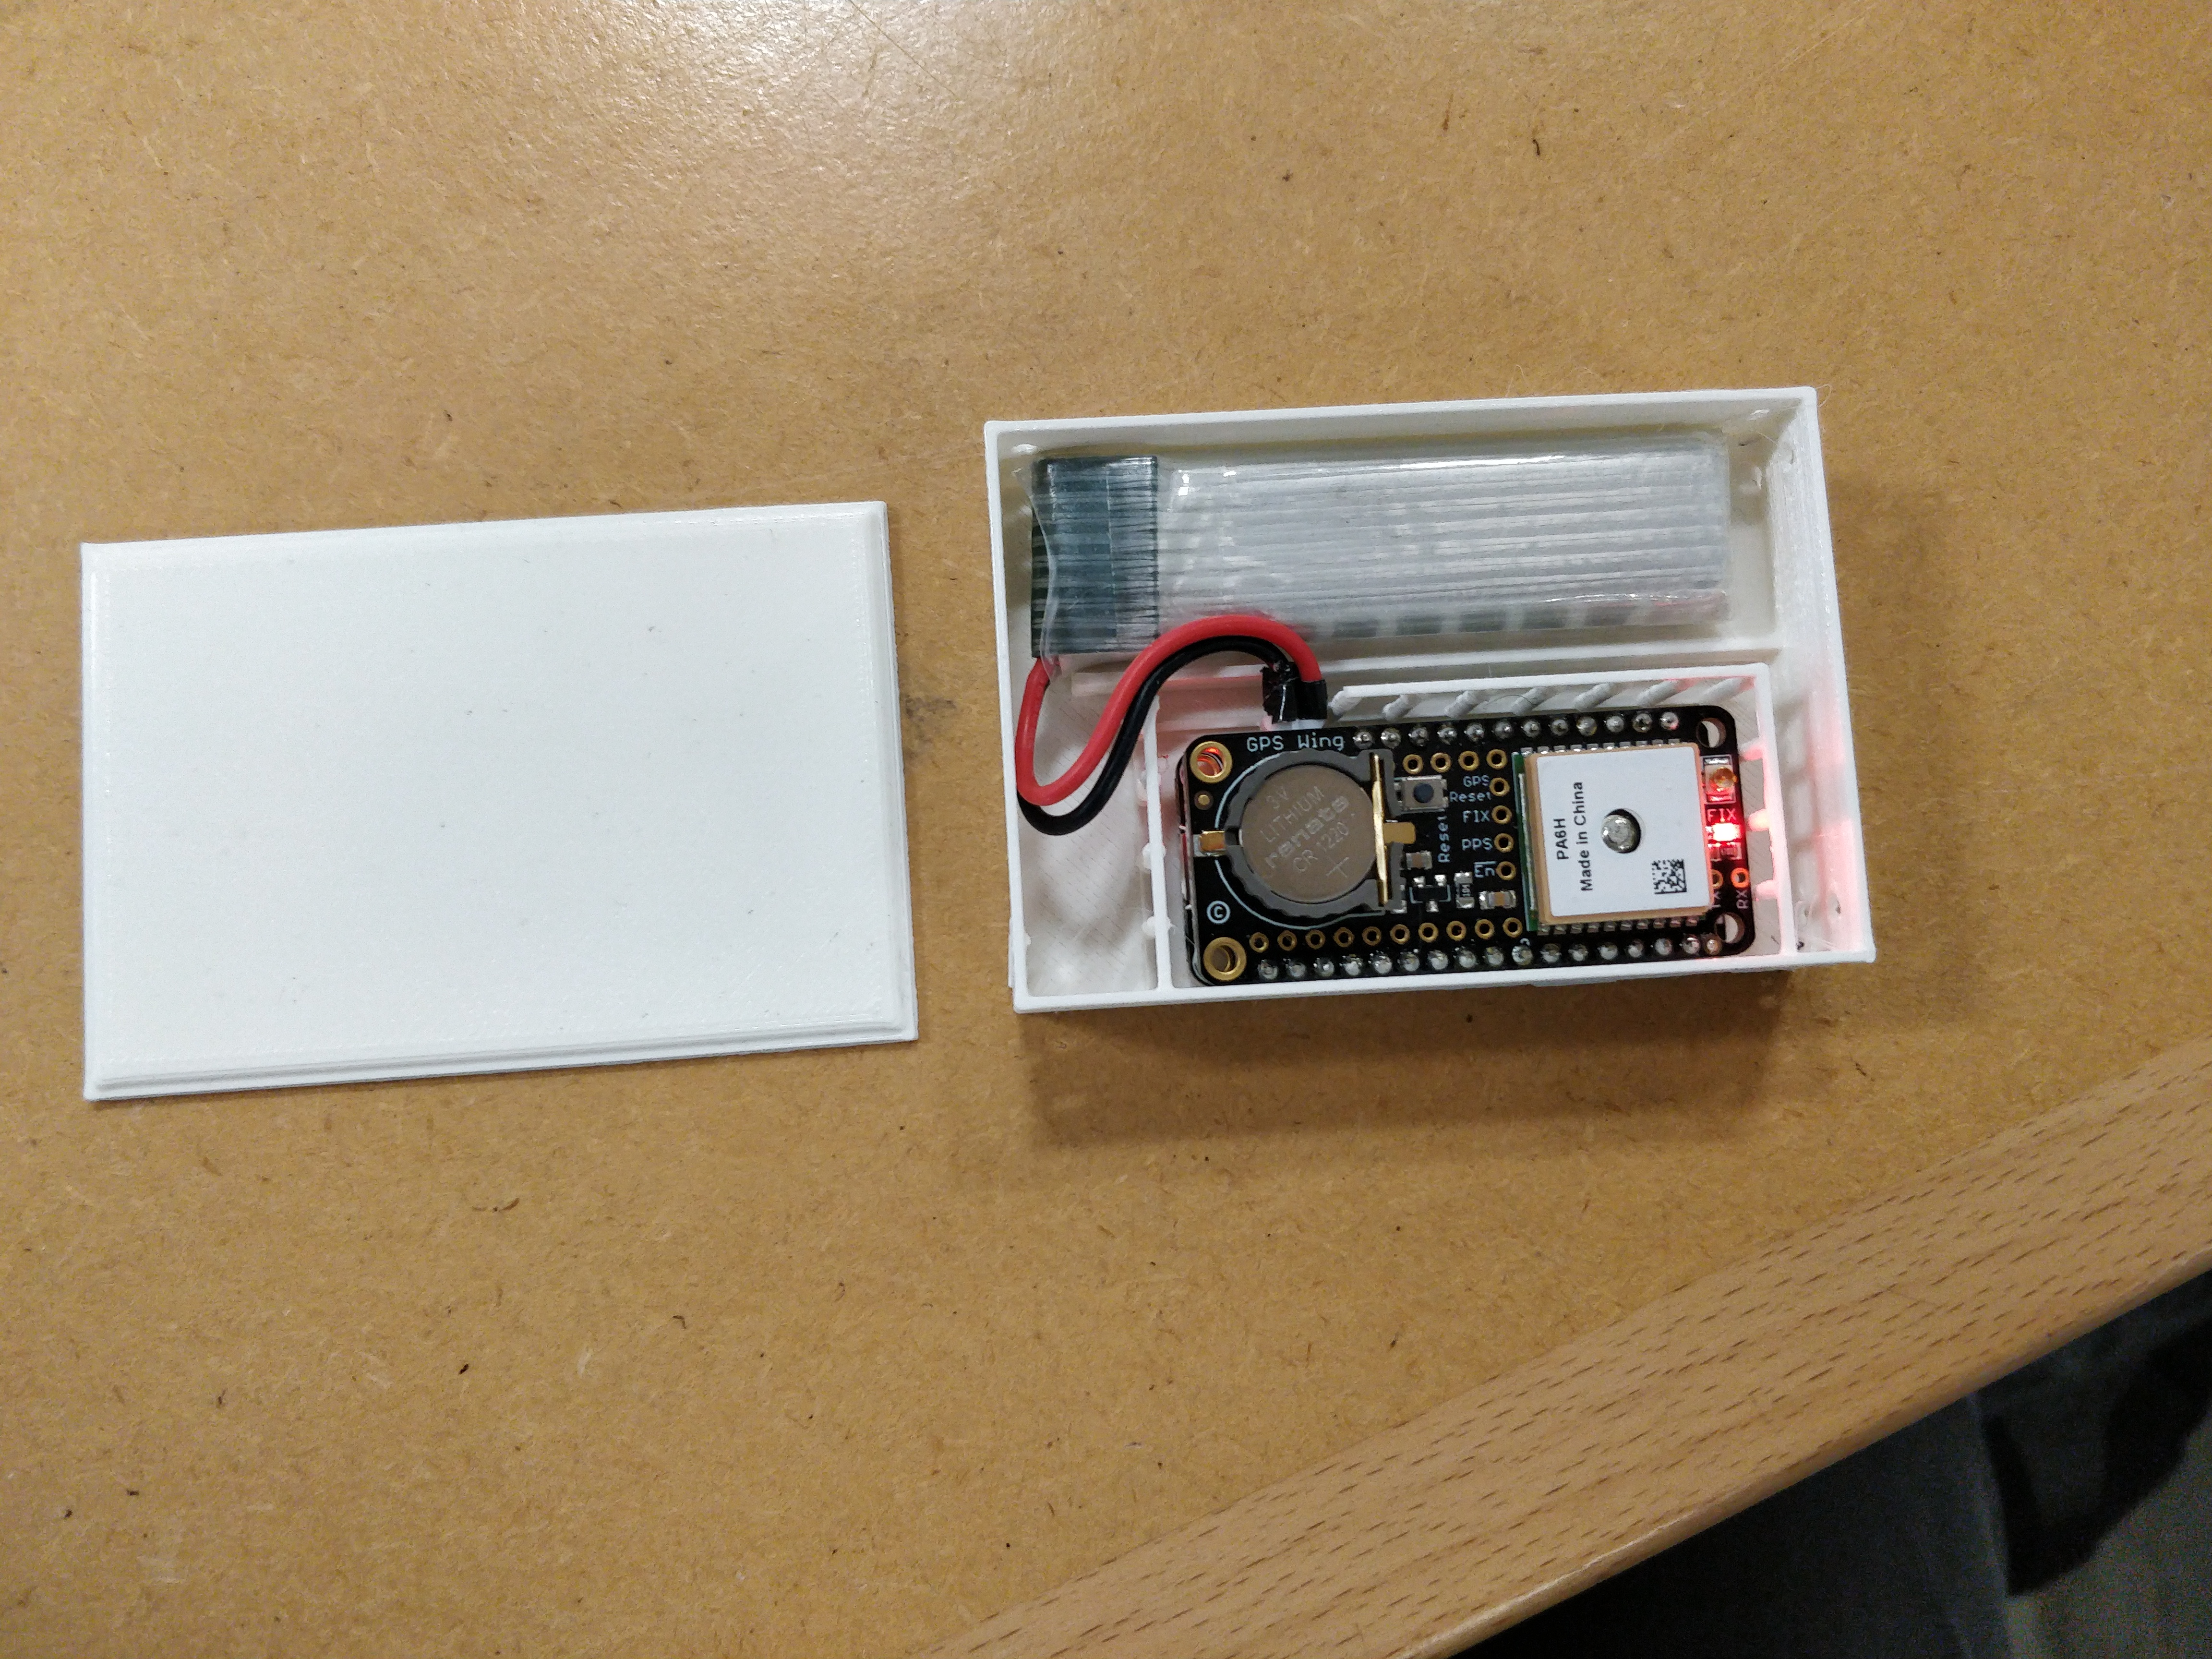
\includegraphics[angle=90,width=\textwidth]{../figures/Pics/firstcase1.jpg}
            \caption{Case overview with lid}
        \end{subfigure}
        \hfill
        \begin{subfigure}[b]{0.4\textwidth}  
            \centering 
            \includegraphics[width=\textwidth]{../figures/Pics/firstcase2.jpg}
            \caption{Battery port view}
        \end{subfigure}
        \vskip\baselineskip
        \begin{subfigure}[b]{0.4\textwidth}   
            \centering 
            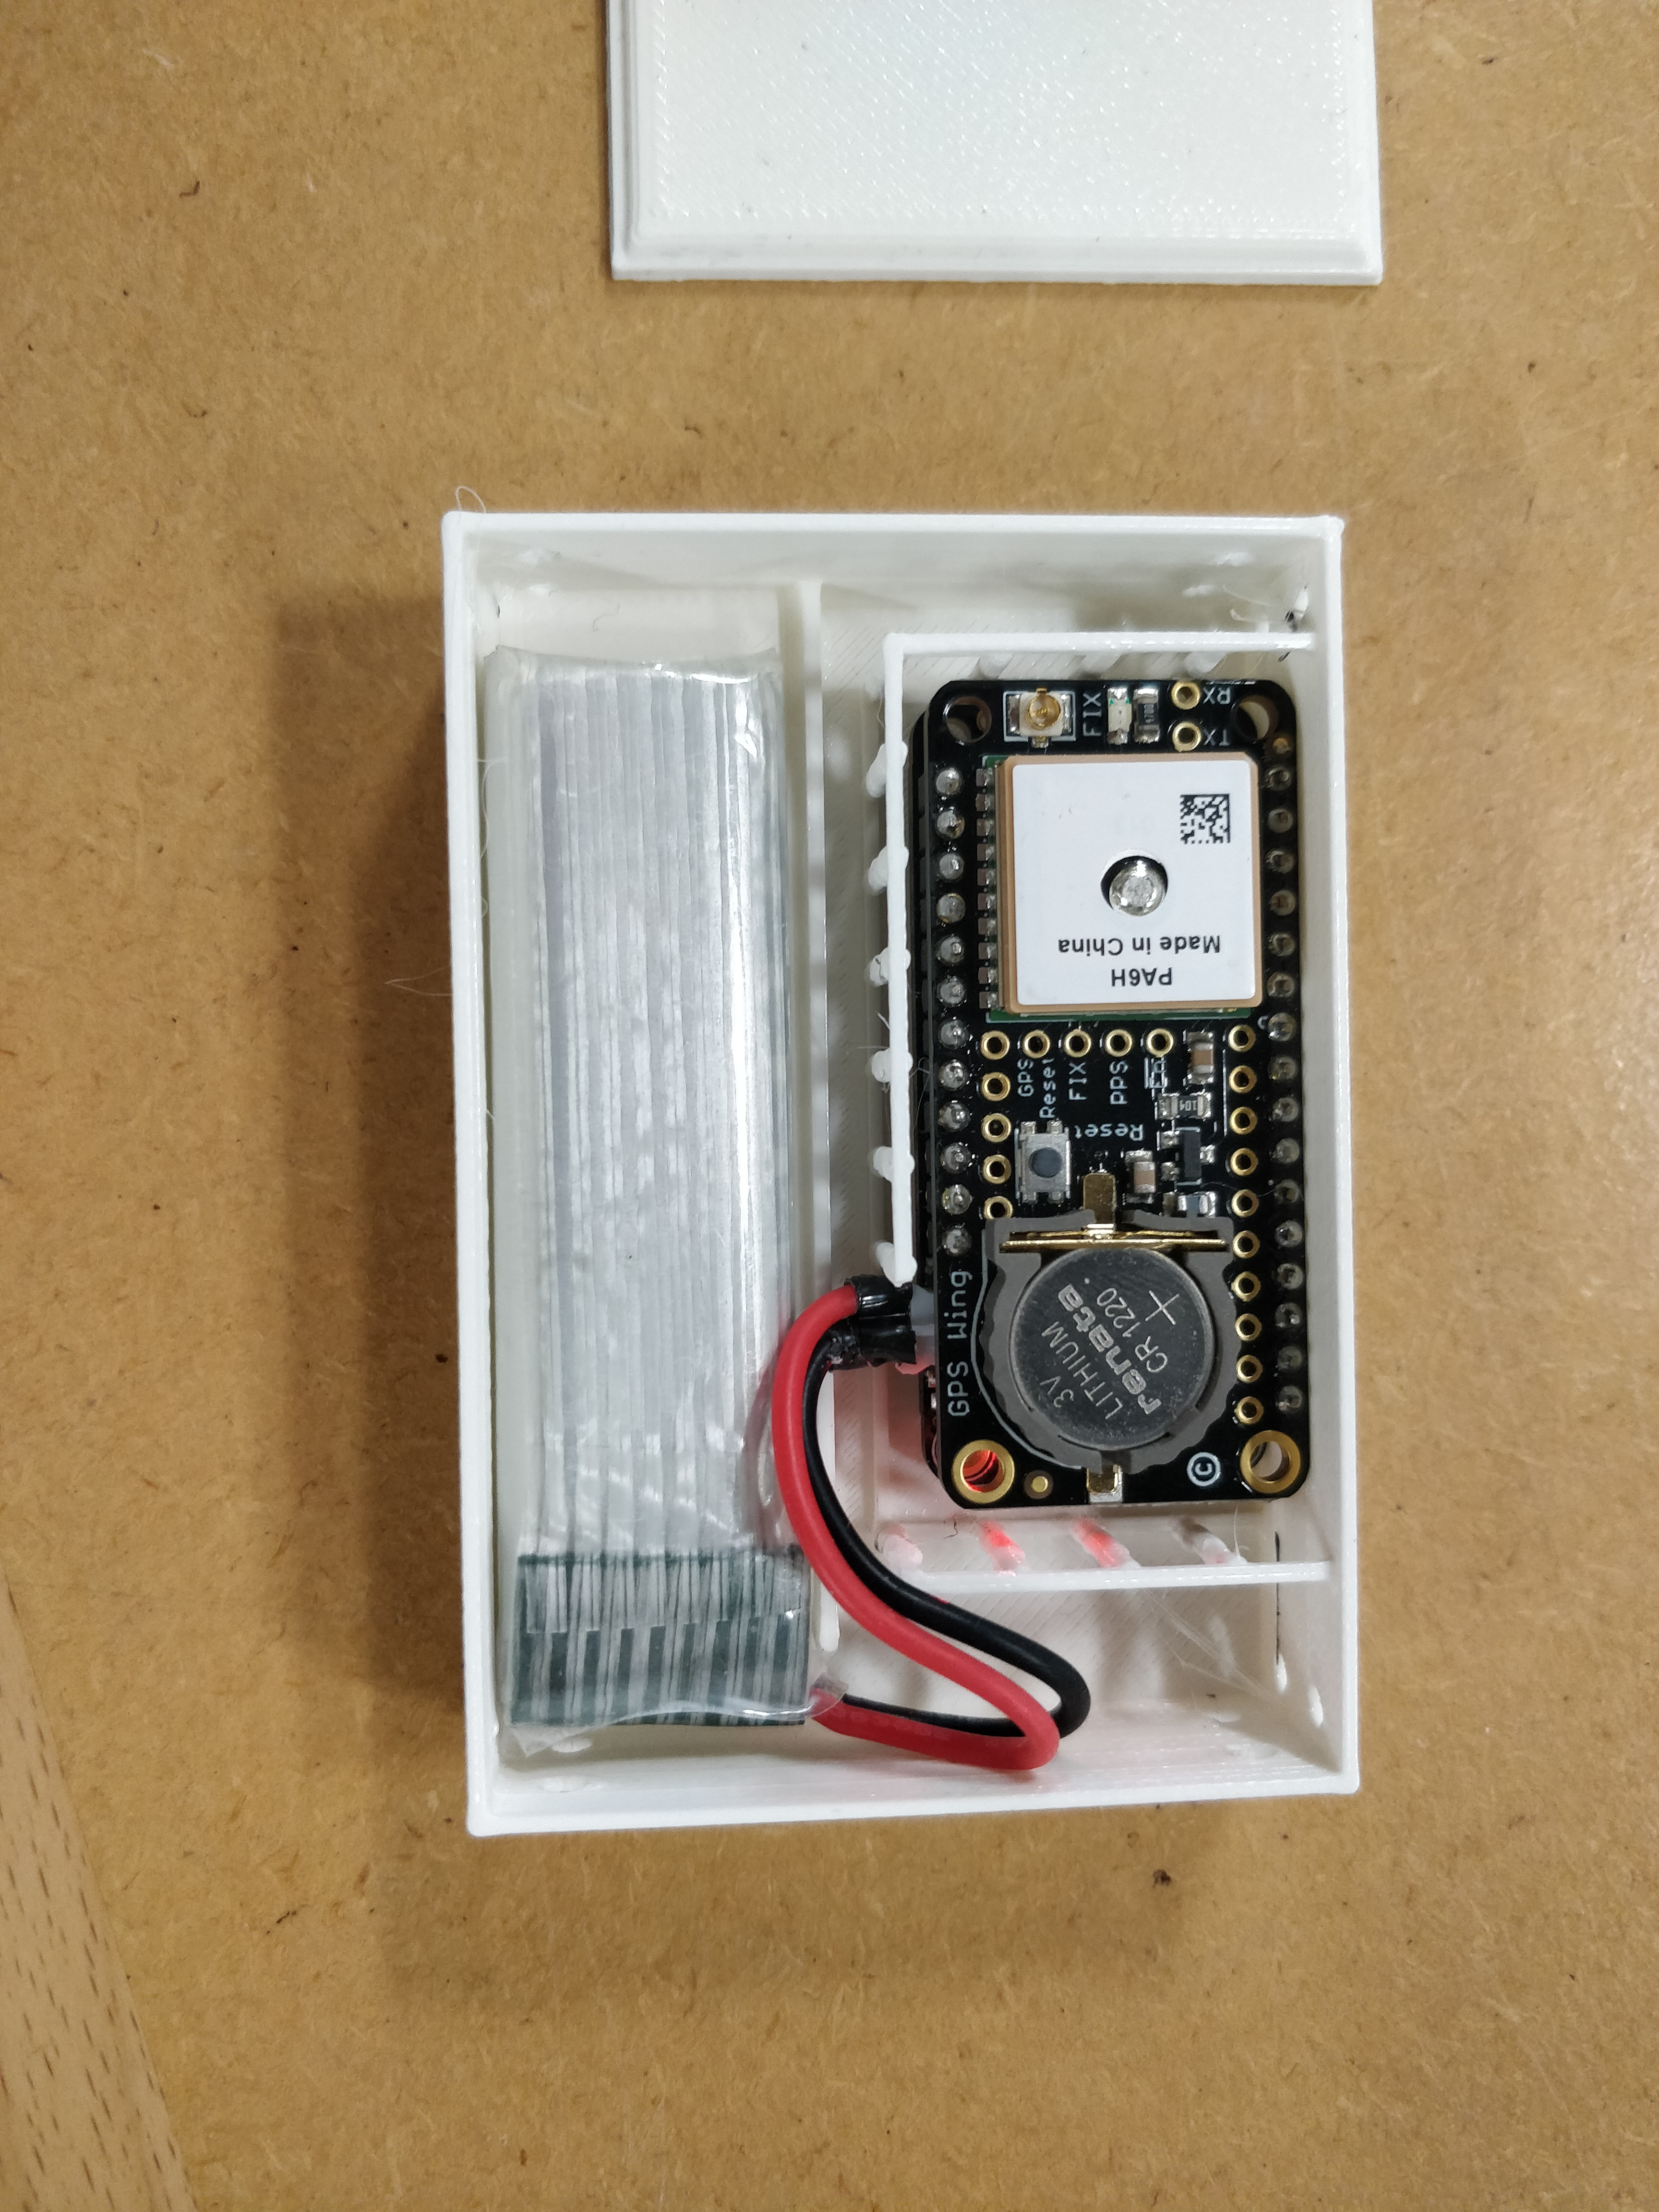
\includegraphics[width=\textwidth]{../figures/Pics/firstcase3.jpg}
            \caption{Top view}            
            \label{fig:case1top}
        \end{subfigure}
        \hfill
        \begin{subfigure}[b]{0.4\textwidth}   
            \centering 
            \includegraphics[width=\textwidth]{../figures/Pics/firstcase4.jpg}
            \caption{Angled front view}
        \end{subfigure}        
    \end{figure}
    \vfill
    \clearpage

    % \begin{figure}[H]        
    %     \label{case1dwg}
    %     \caption{Case 1 dimensional drawing}
    %     \includegraphics[angle=-90,width=\textwidth]{../../Design/case1.pdf}
    % \end{figure}  

    % \includepdf[pagecommand={},angle=-90,scale=0.9,pagecommand=\section{Case 1 dimensional drawing \label{fig:case1dwg}}]{../../Design/case1.pdf}  
    
    \begin{figure}[H]      
        \caption{Case 1 dimensional drawings}
        \includepdf[pagecommand={},angle=-90,scale=0.9]{../../Design/case1.pdf}  
        \label{fig:case1dwg}
    \end{figure}
    % \clearpage
       
    % \section{Case 2 images}
    \vfill
    \begin{figure}[H]          
        \caption[Second case print]{Second case print, showing various angles} 
        \label{fig:case2img}  
        \centering
        \begin{subfigure}[b]{0.6\textwidth}  
            \centering 
            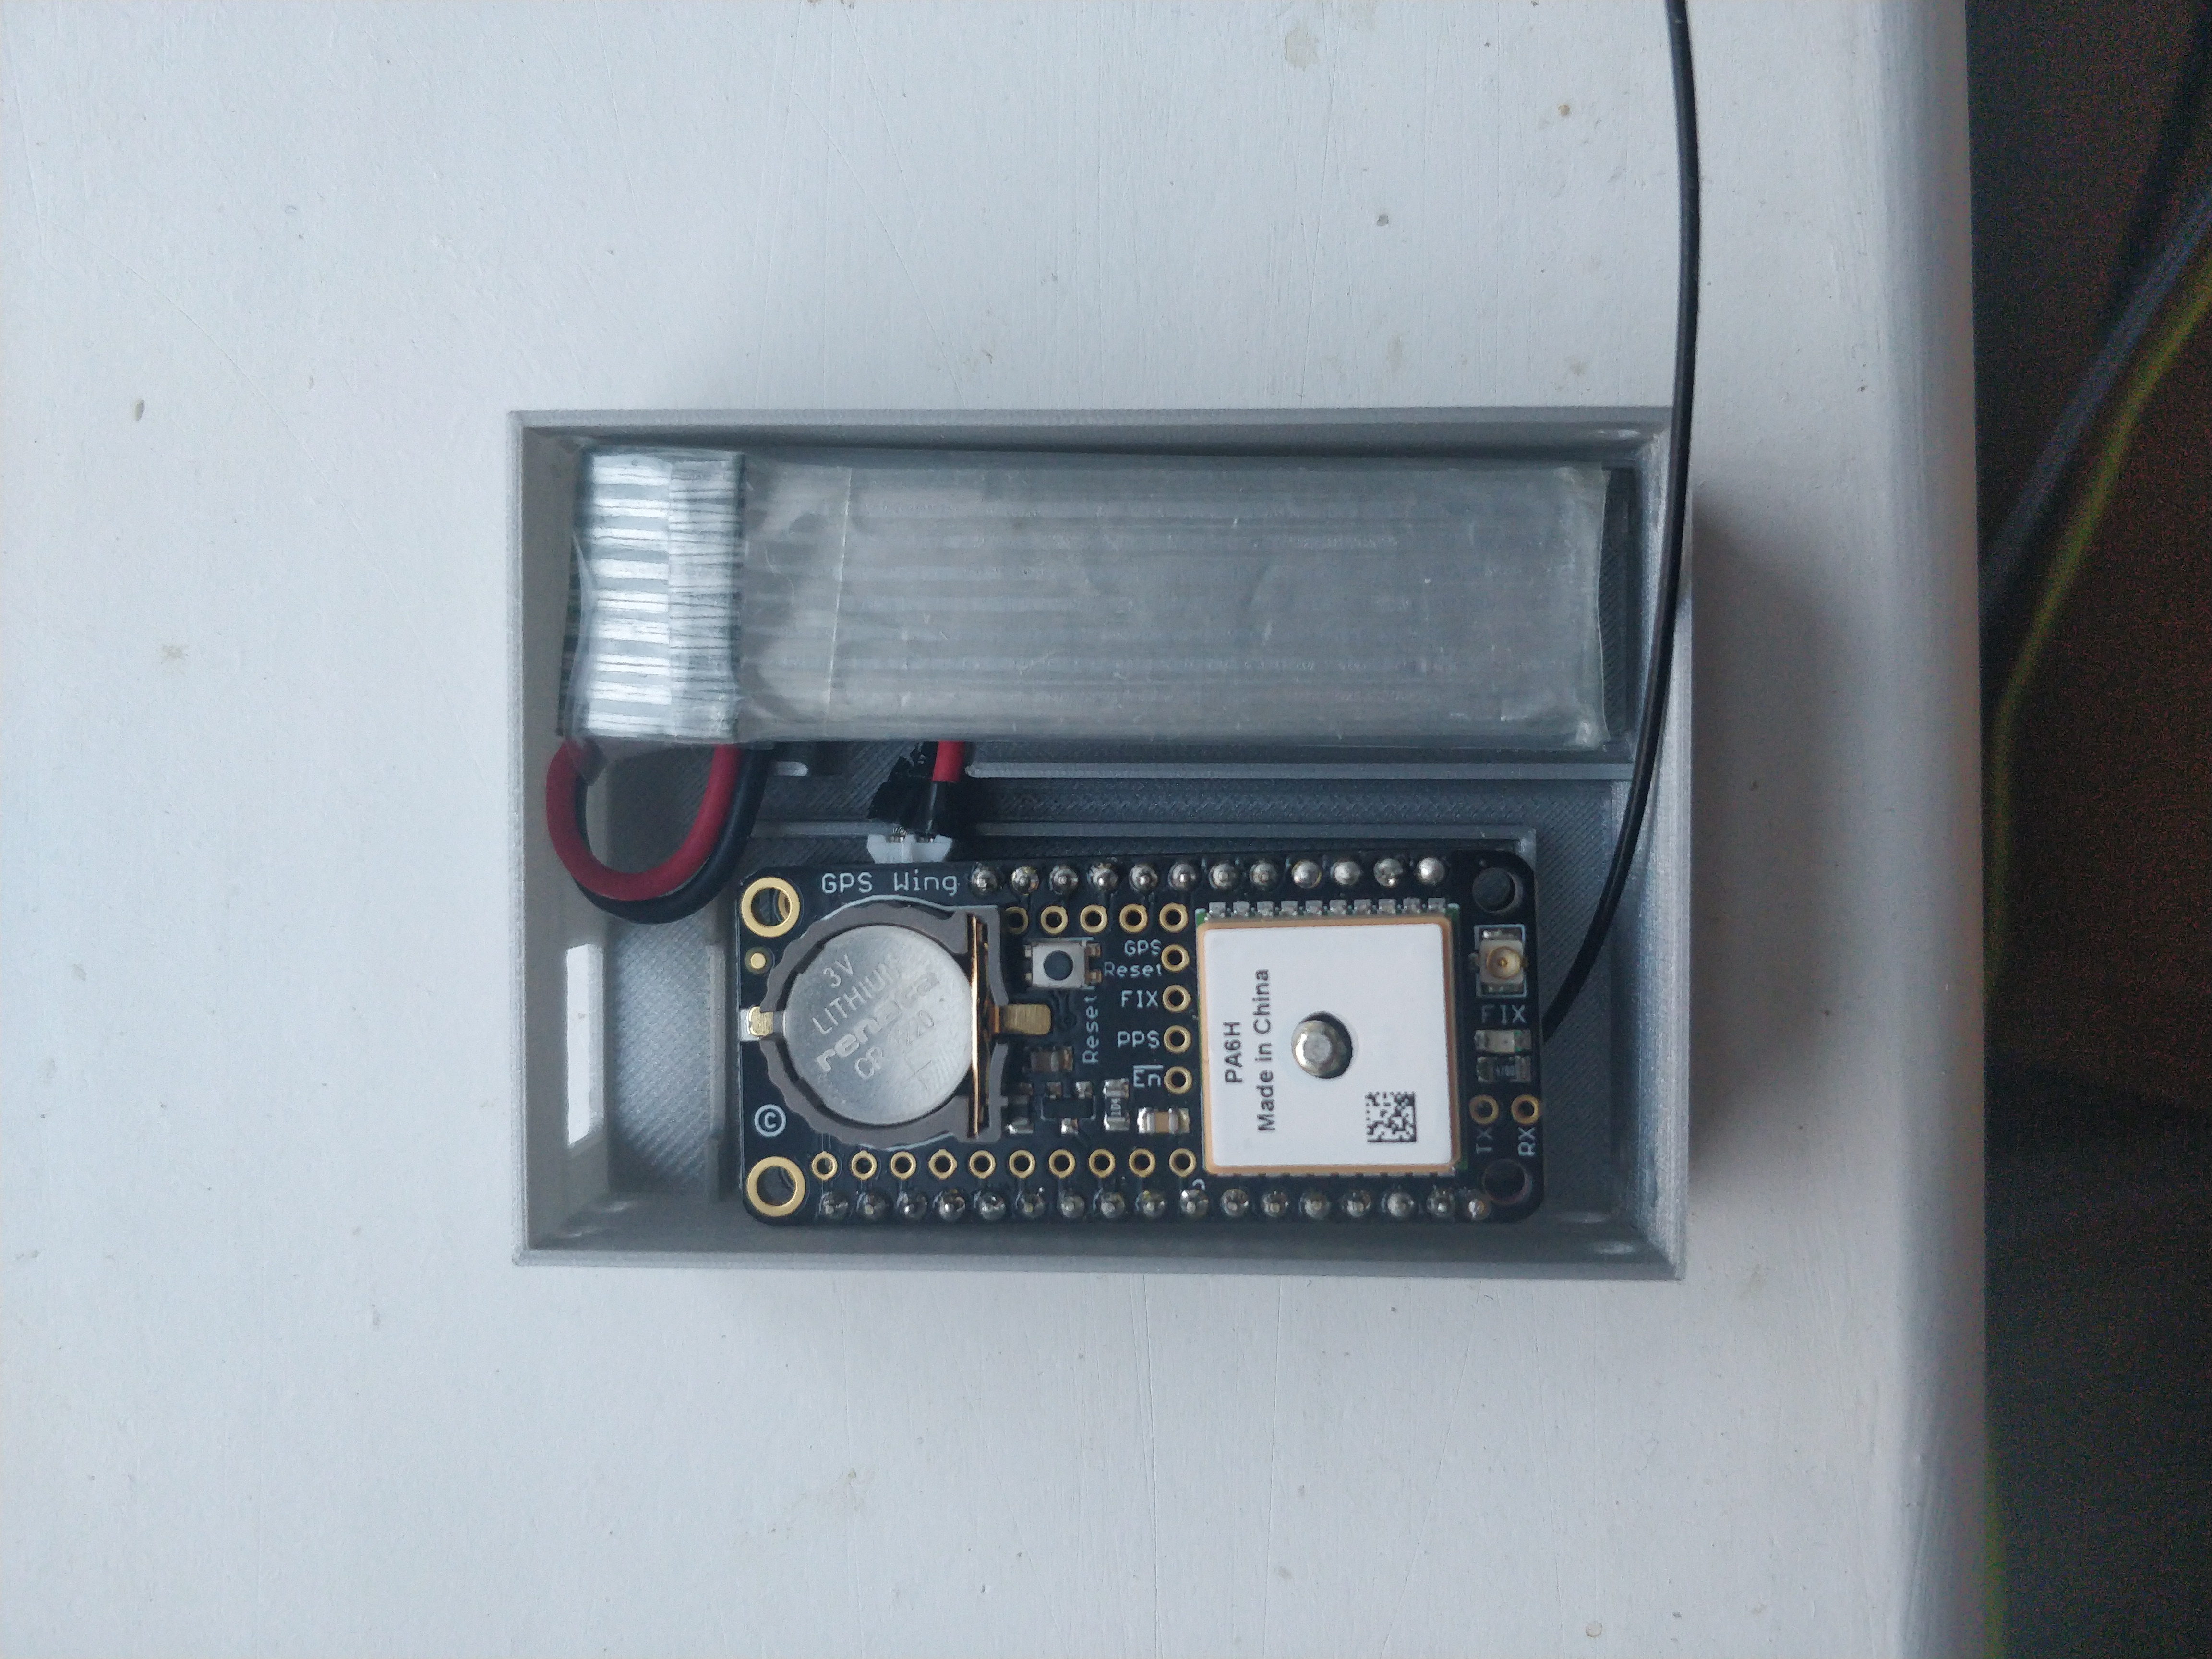
\includegraphics[width=\textwidth]{../figures/Pics/secondcase0.jpg}
            \caption{Case overview}
        \end{subfigure}
        \vskip\baselineskip
        \hspace*{\fill}
        \begin{subfigure}[b]{0.3\textwidth}
            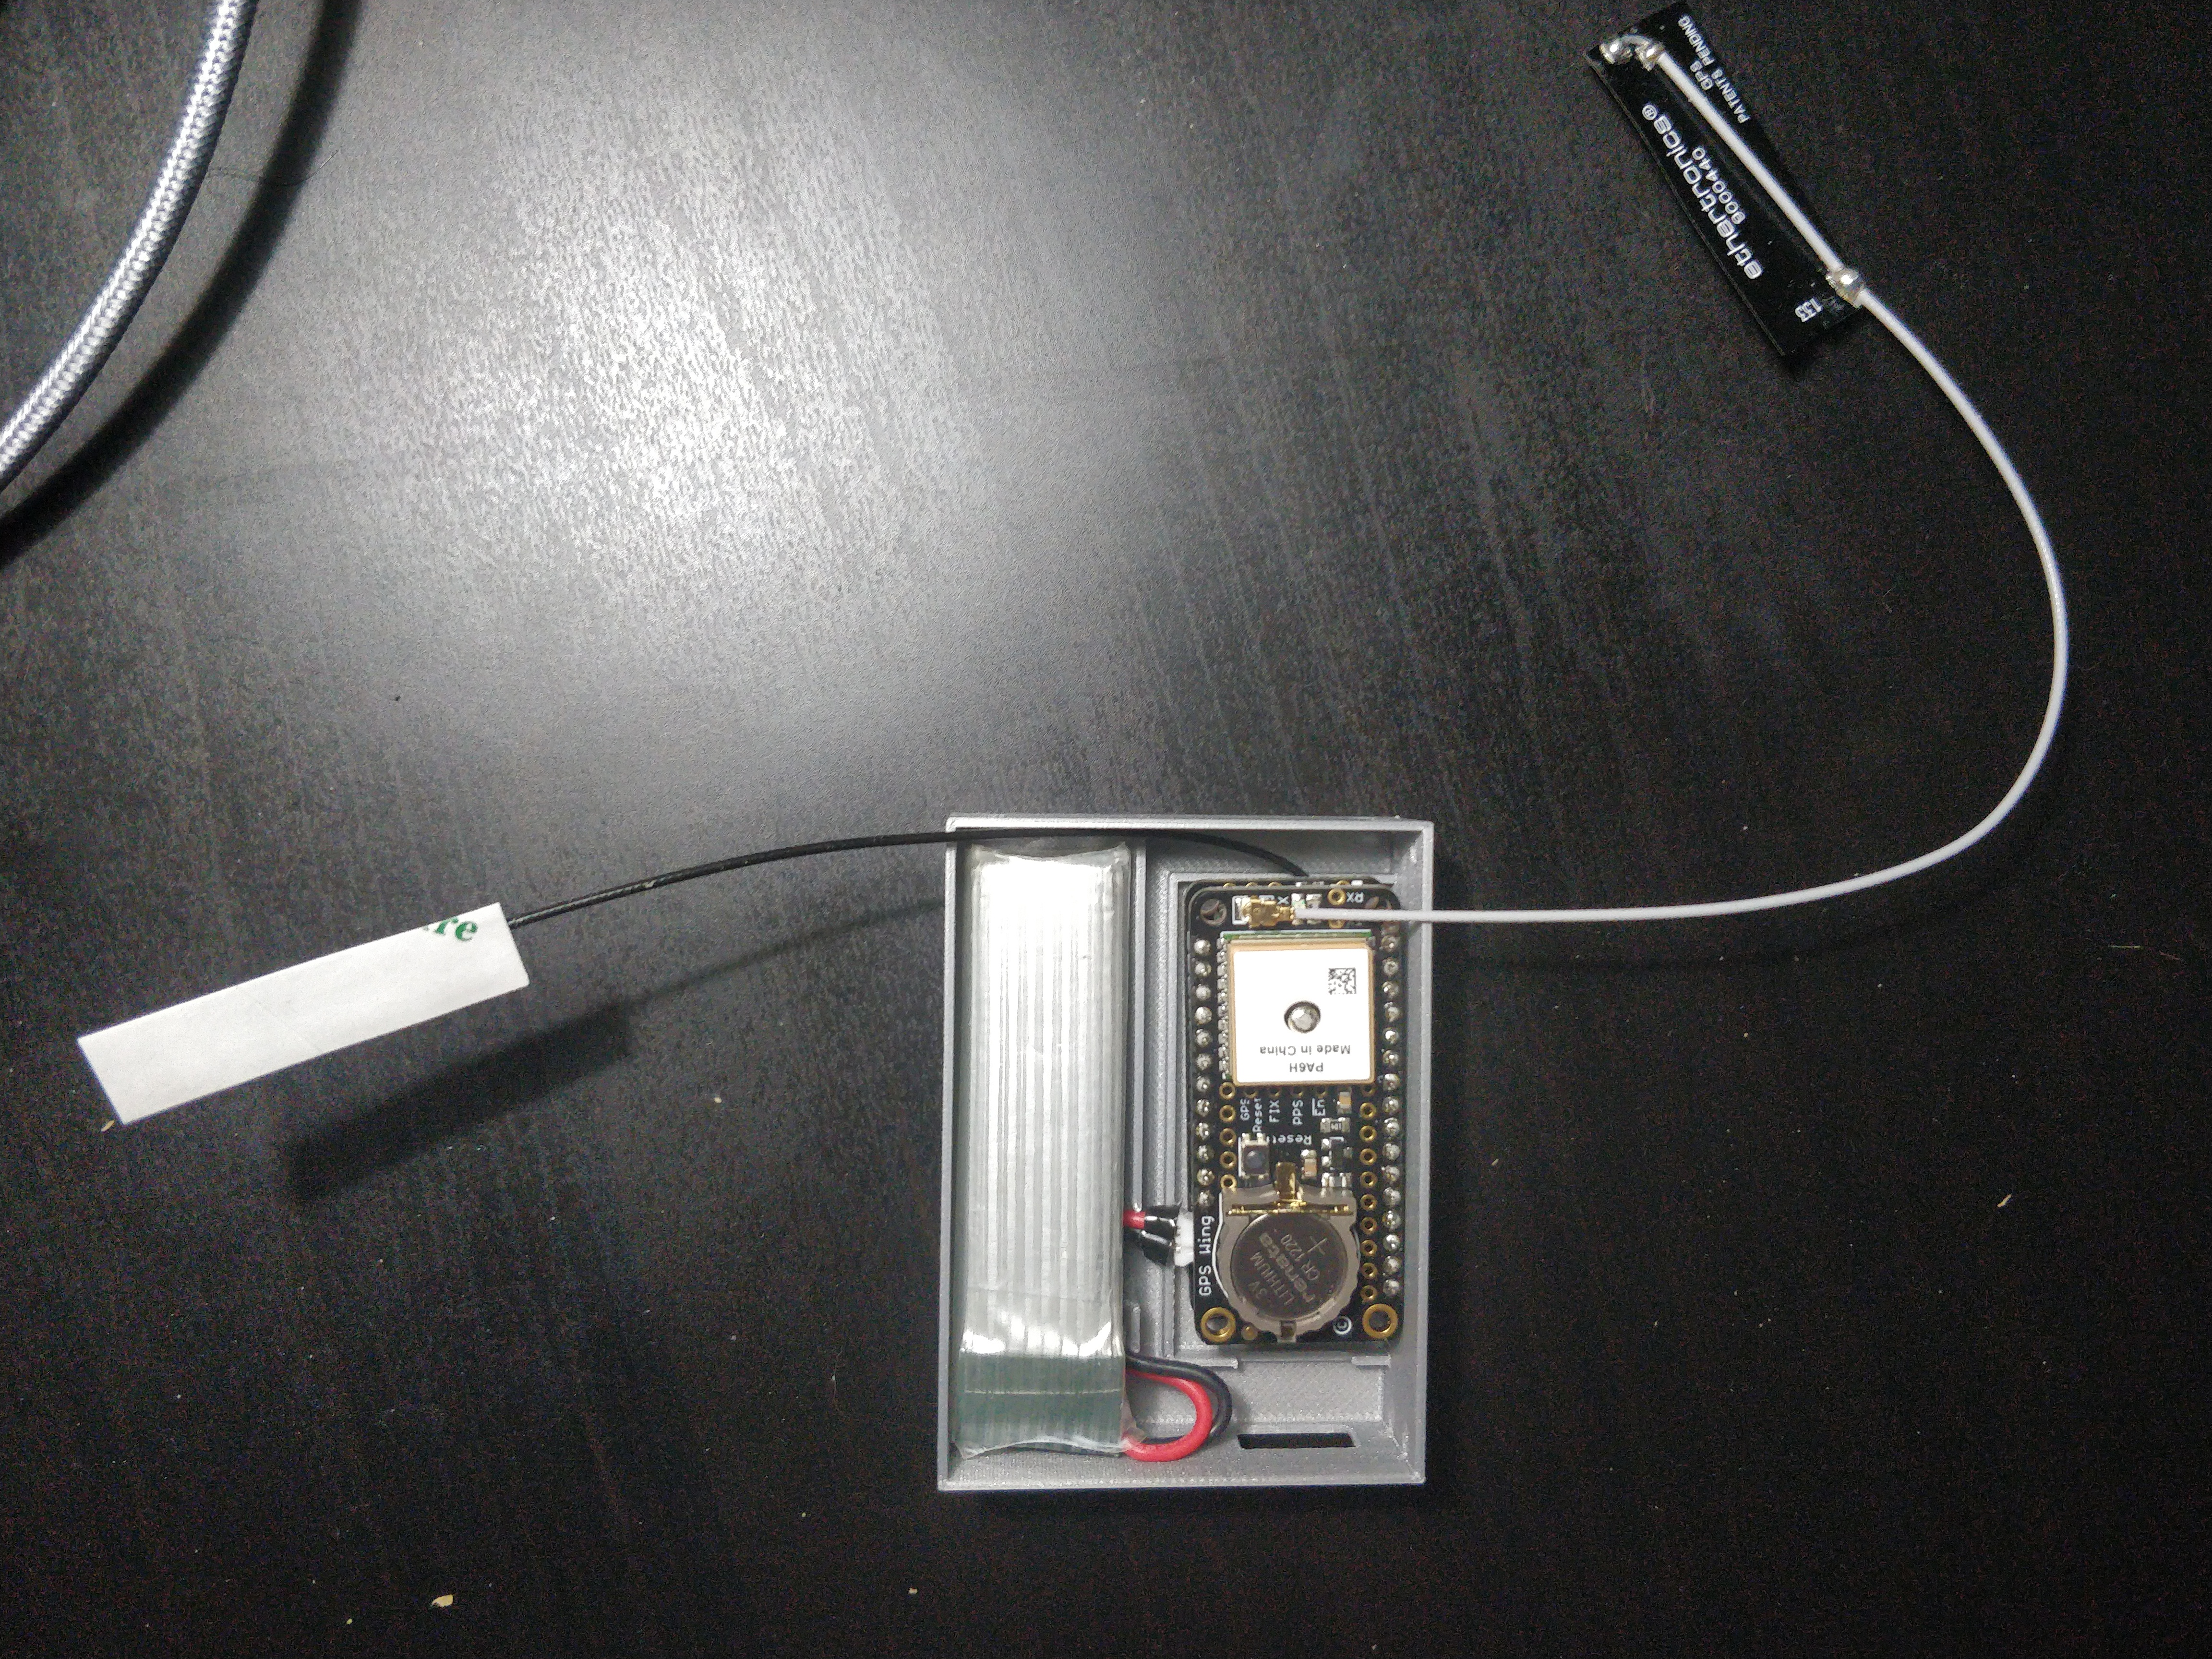
\includegraphics[angle=90,width=\textwidth]{../figures/Pics/secondcase1.jpg}
            \vspace{5pt}
            \caption{Case with antennae}            
            \label{fig:case2antennasplay}
        \end{subfigure}
        \hfill
        \begin{subfigure}[b]{0.3\textwidth}  
            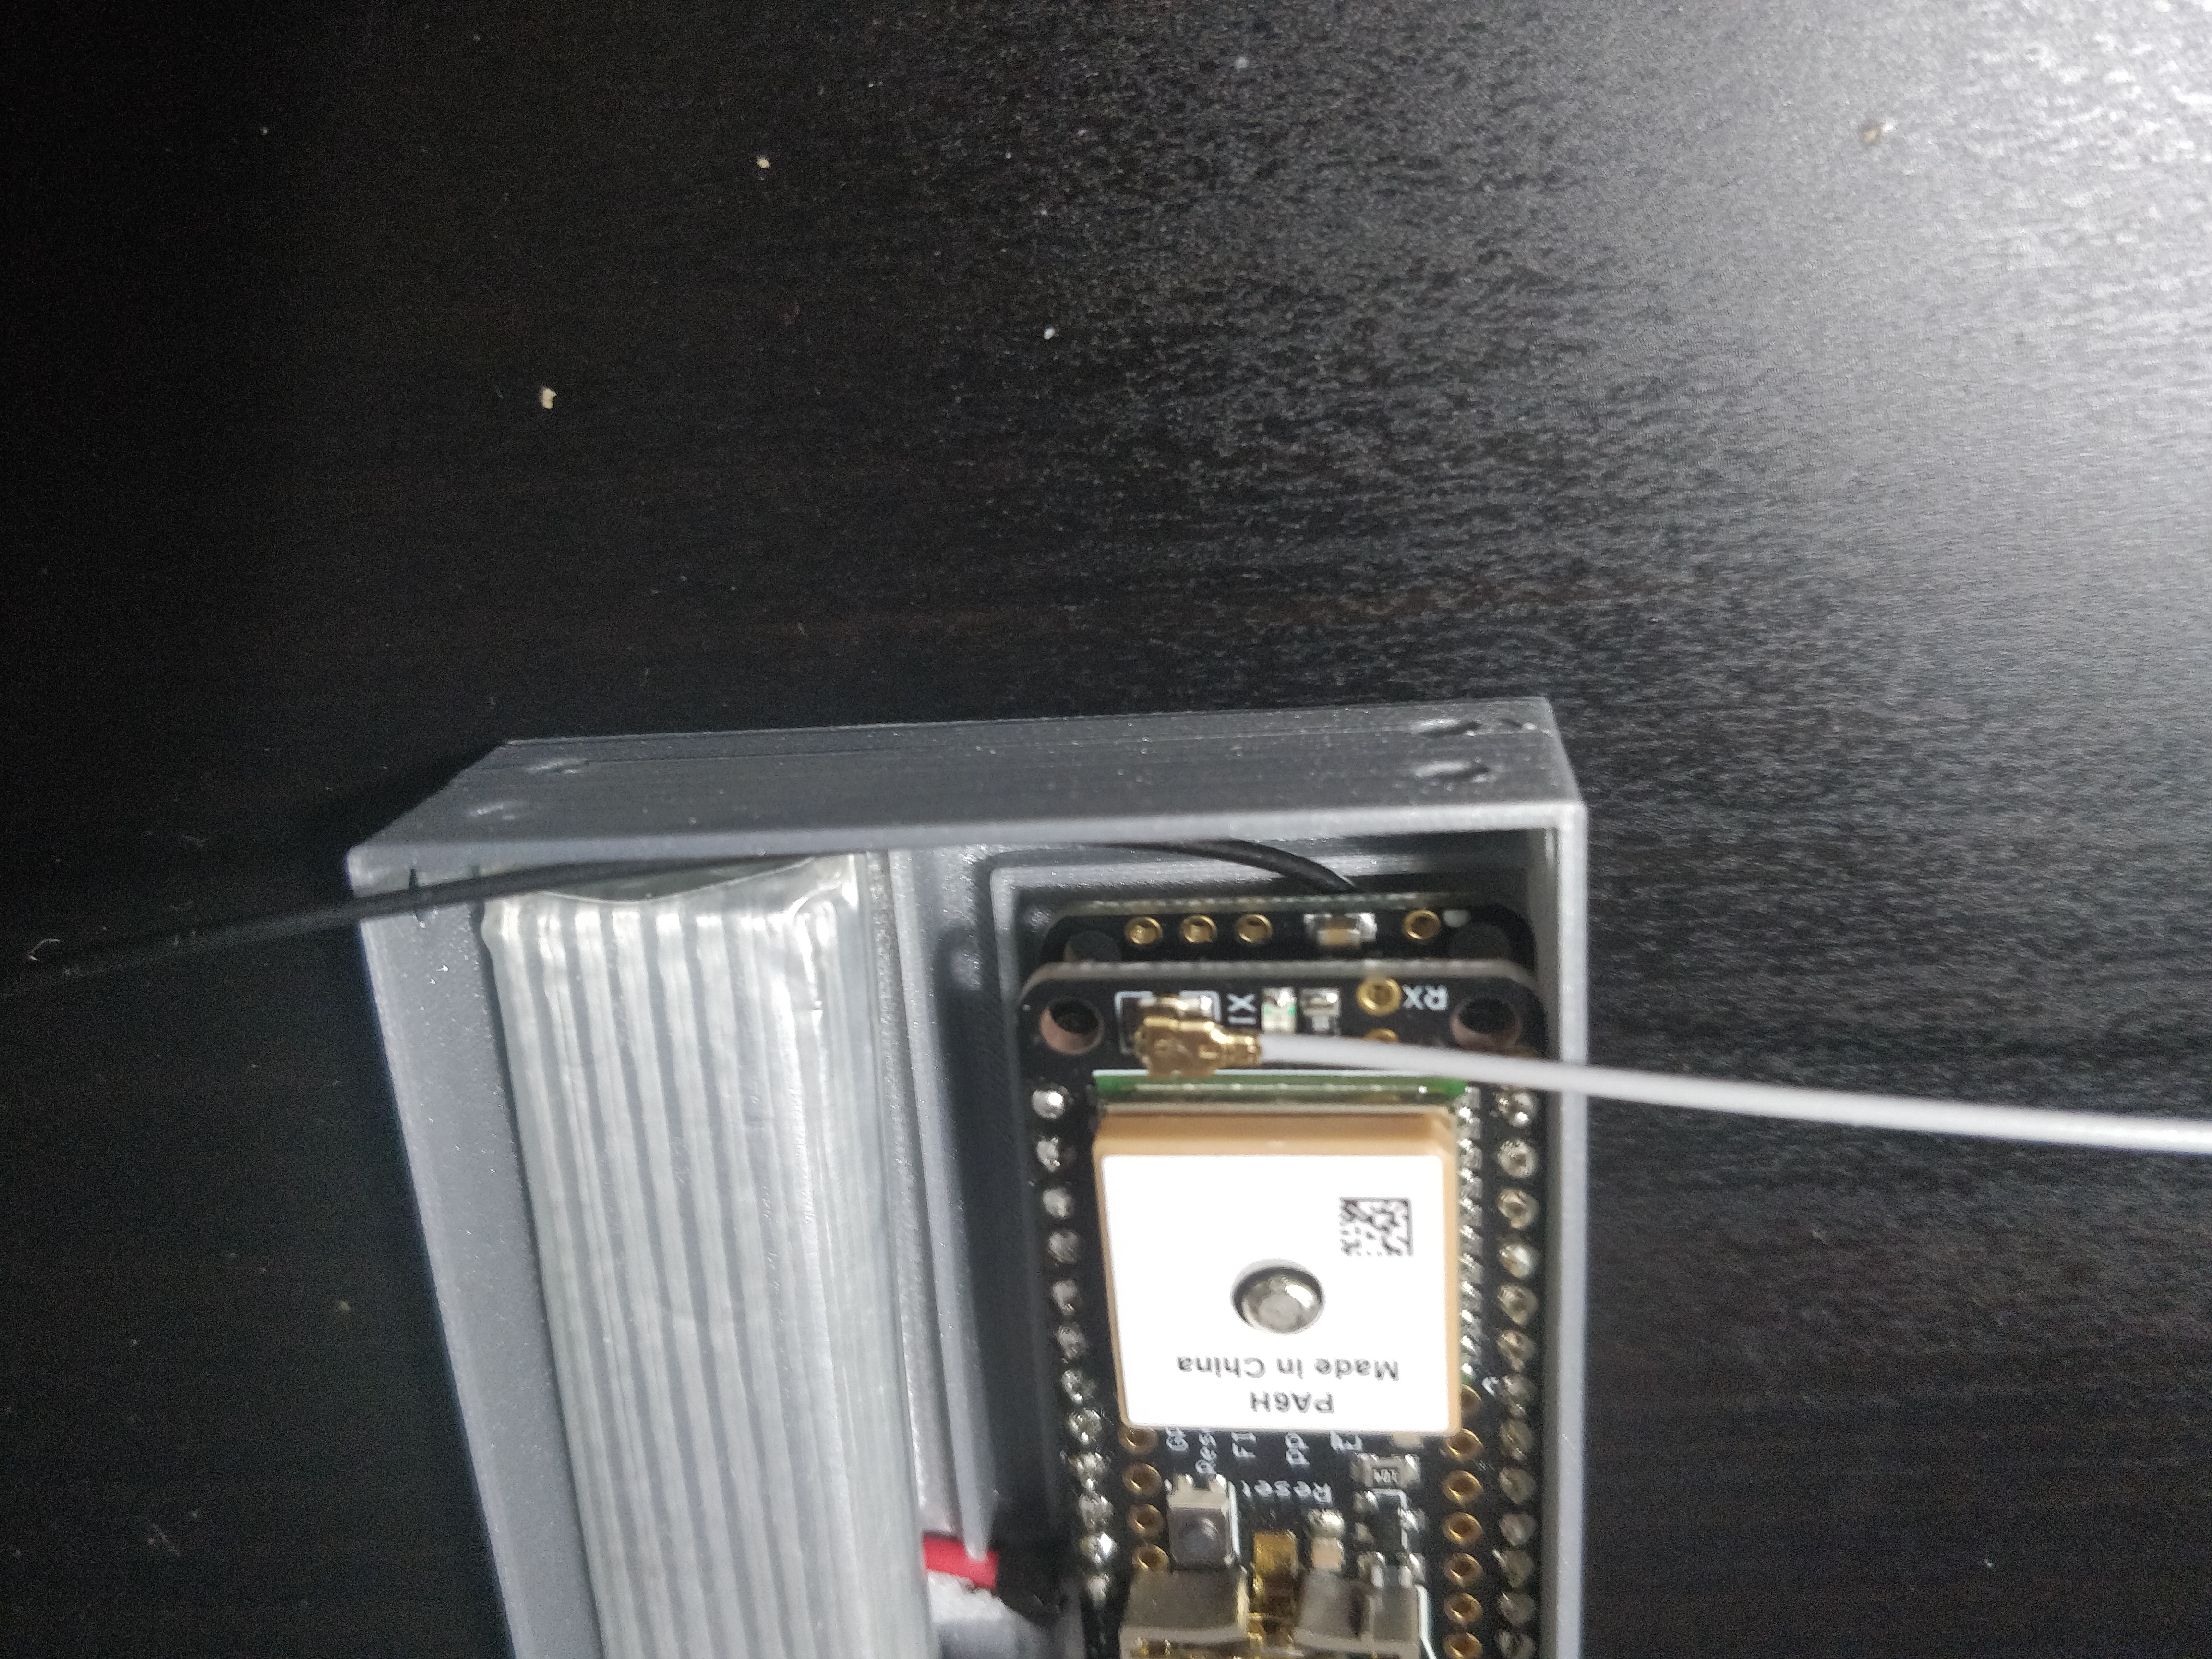
\includegraphics[angle=90,width=\textwidth]{../figures/Pics/secondcase2.jpg}
            \vspace{5pt}
            \caption{Antenna raising issue}                    
            \label{fig:case2antennaissue}
        \end{subfigure}
        \hspace*{\fill}
        \vskip\baselineskip
        \hspace*{\fill}
        \begin{subfigure}[b]{0.3\textwidth}   
            \captionsetup{justification=centering}
            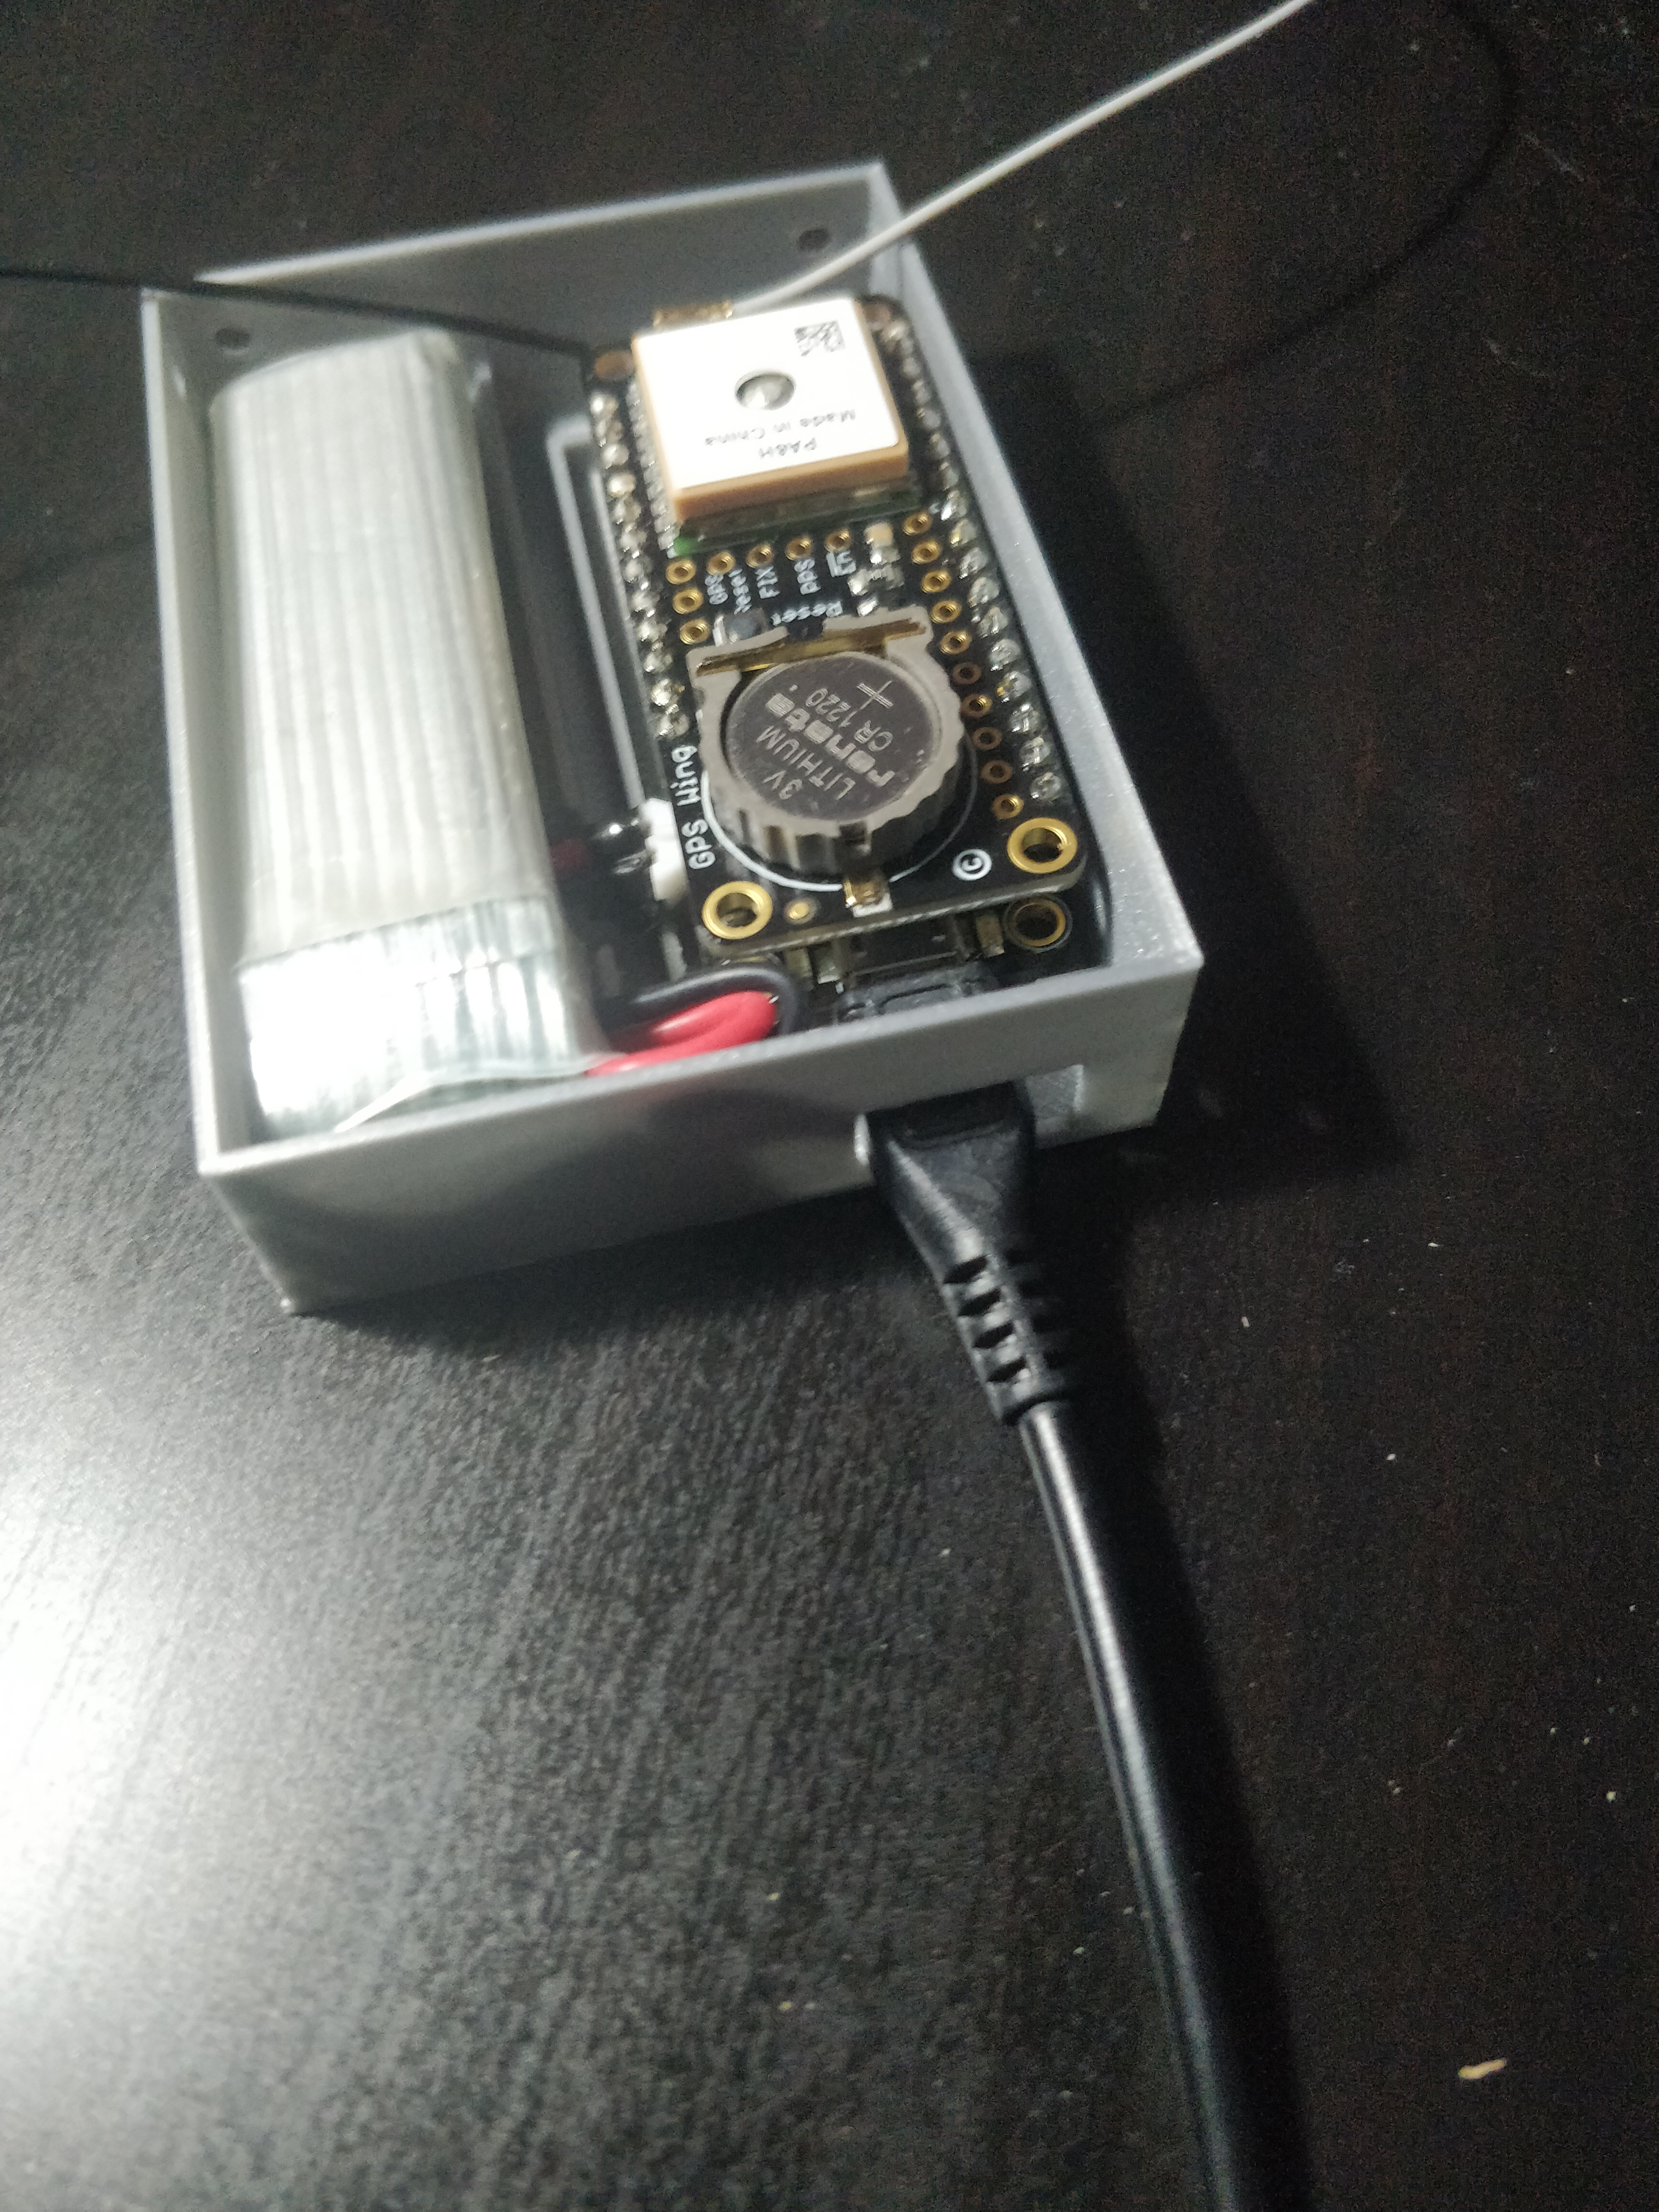
\includegraphics[width=\textwidth]{../figures/Pics/secondcase3.jpg}
            \vspace{1pt}
            \caption{Angled front view with \acrshort{usb} connection}
        \end{subfigure}
        \hfill
        \begin{subfigure}[b]{0.3\textwidth}           
            \captionsetup{justification=centering}
            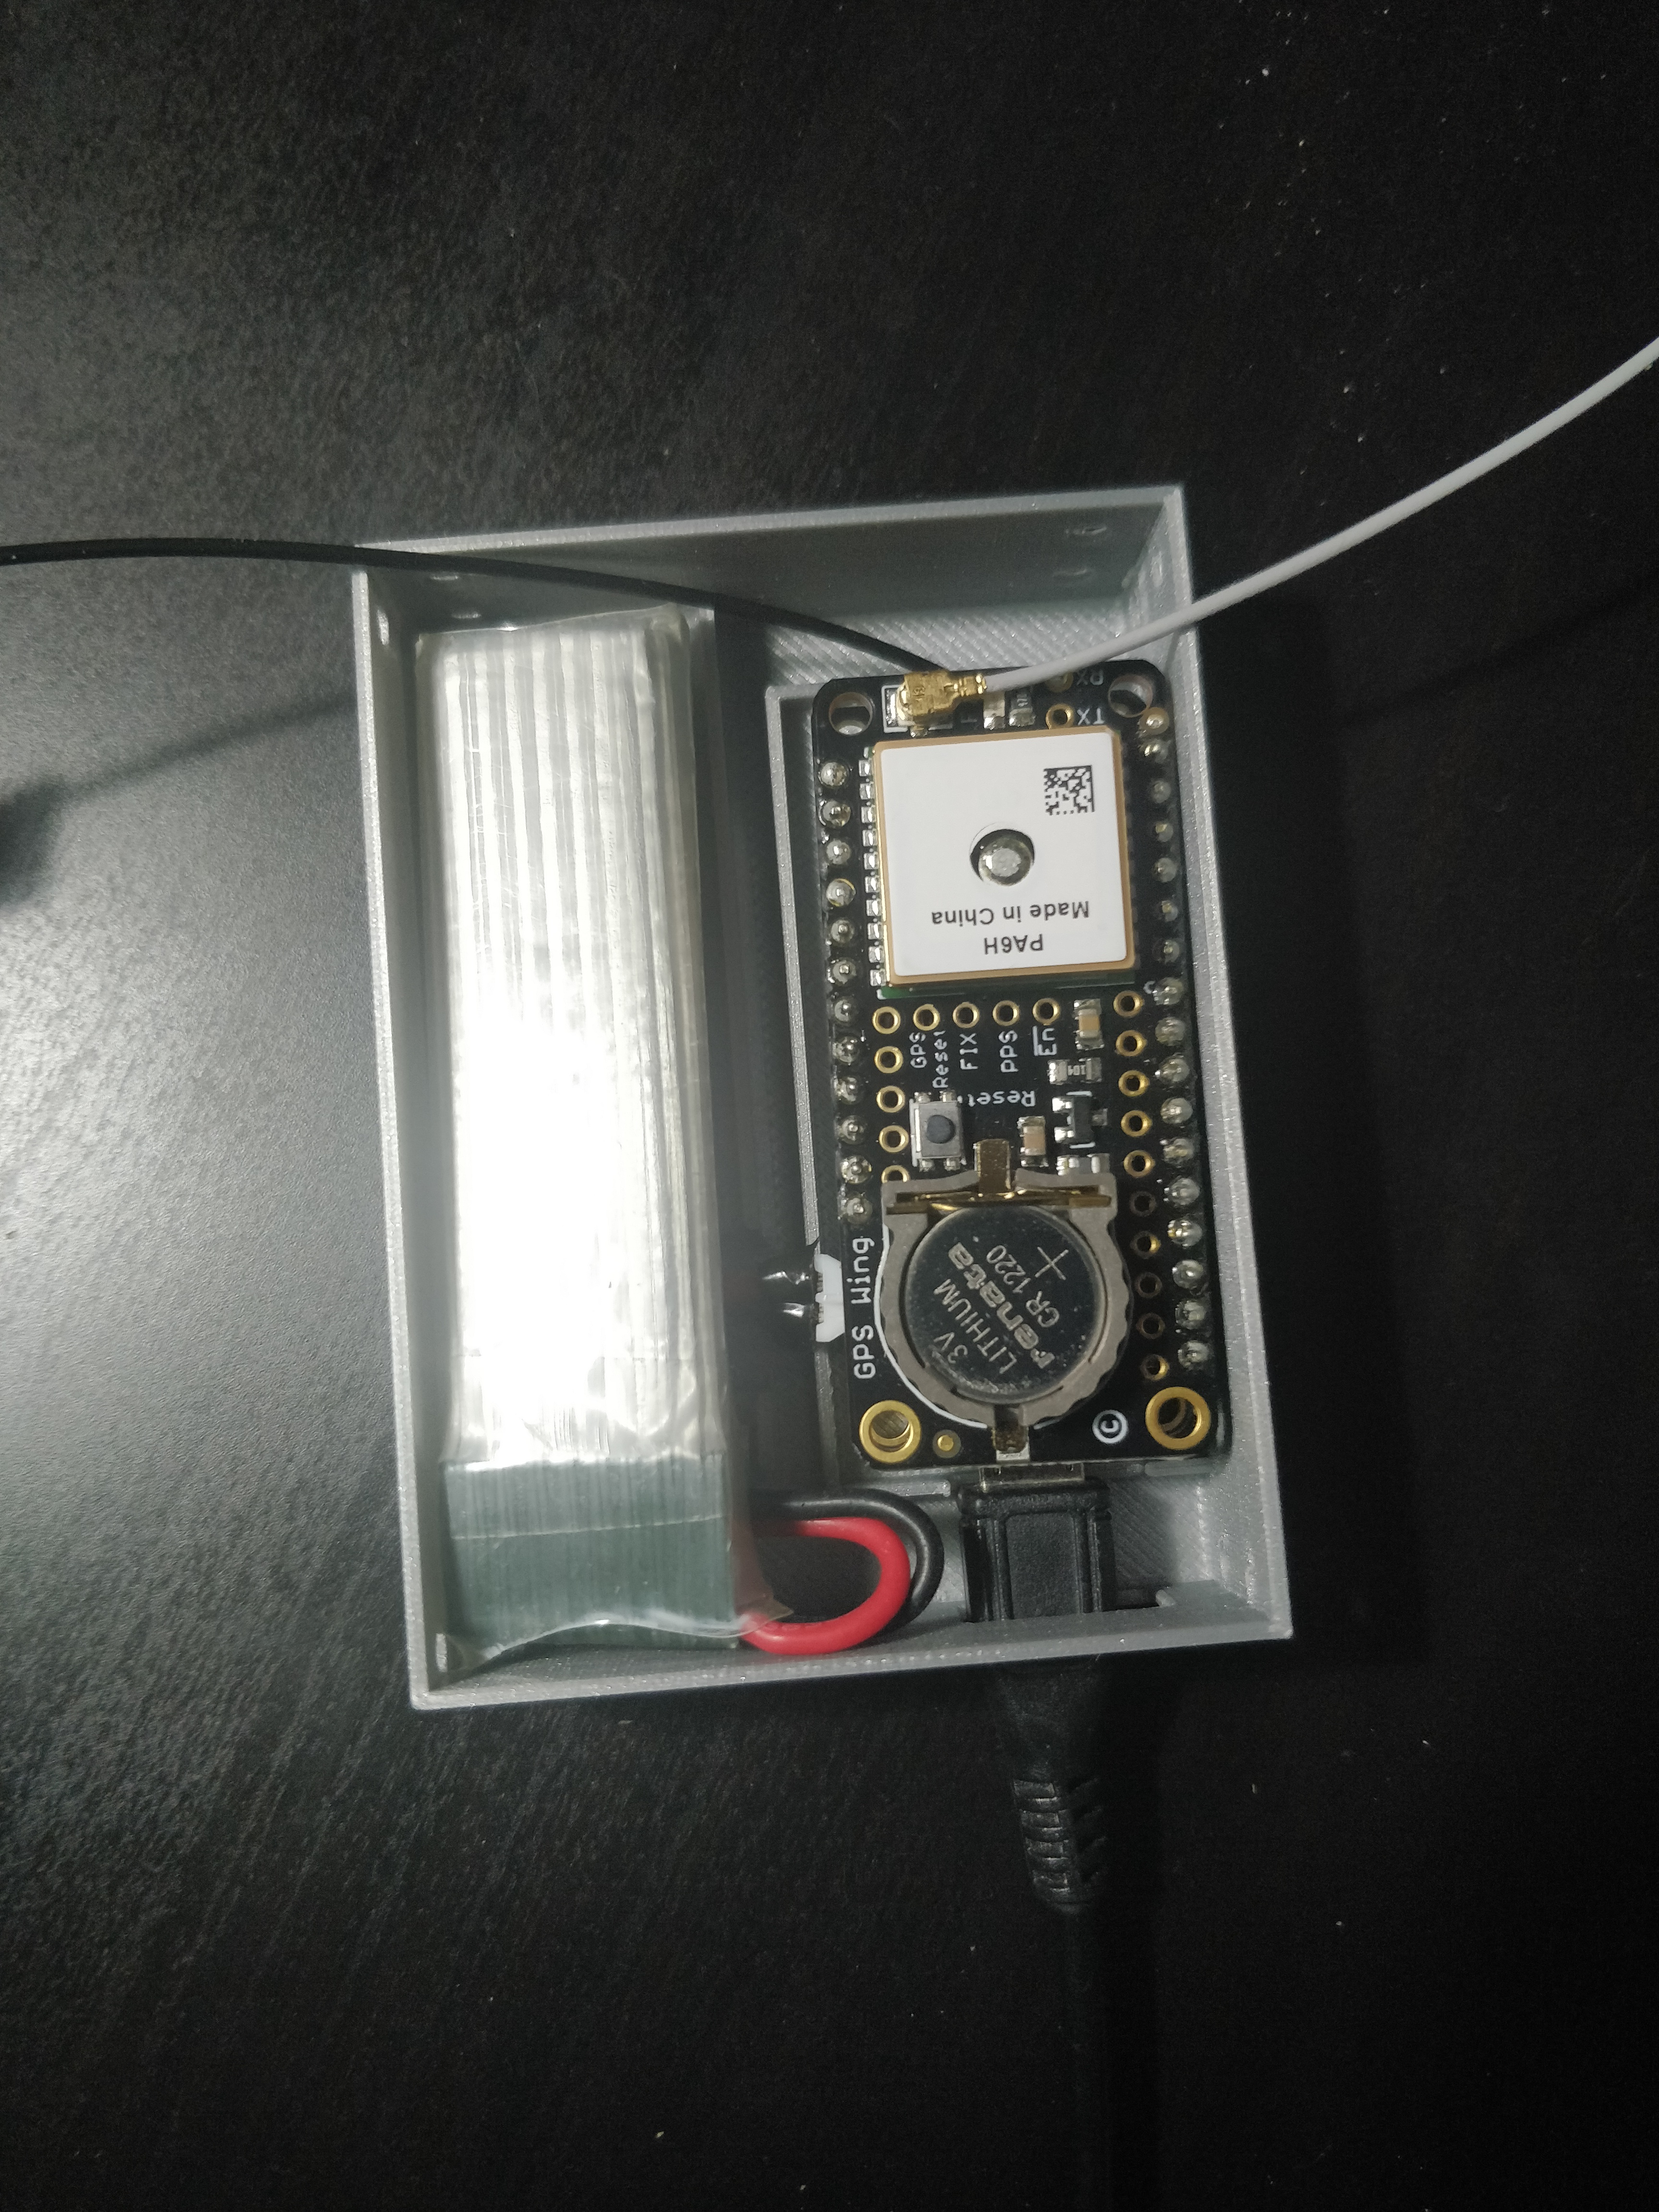
\includegraphics[width=\textwidth]{../figures/Pics/secondcase4.jpg}
            \vspace{5pt}
            \caption{Top view with \acrshort{usb} connection}
        \end{subfigure}
        \hspace*{\fill}
    \end{figure}
    \vfill
    \clearpage

    % \begin{figure}[H]        
    %     \label{case2dwg}
    %     \caption{Case 2 dimensional drawing}
    %     \includegraphics[angle=-90,width=\textwidth]{../../Design/case2.pdf}
    % \end{figure}   

    % \begin{figure}[H]        
        % \includepdf[pagecommand={},angle=-90,scale=0.9,pagecommand=\section{Case 2 dimensional drawing \label{fig:case2dwg}}]{../../Design/case2.pdf}
        % \label{fig:case2dwg}
    % \end{figure}
    % \clearpage

    \begin{figure}[H]      
        \caption{Case 2 dimensional drawings}
        \includepdf[pagecommand={},angle=-90,scale=0.9]{../../Design/case2.pdf}  
        \label{fig:case2dwg}
    \end{figure}
   


\begin{landscape}

\chapter{Purchasing lists}

    \begin{xltabular}{\linewidth}{|cYccccc|}
        \caption{Preliminary hardware list} \label{table:prelimhardwarelist} \\
        \hline

        \rowcolor{tableh2}
        Part & Description & Quantity  & Price per unit & Supplier & SKU & Web link \\
        \endfirsthead

        \caption{Preliminary hardware list (cont.)}\\
        \hline
        \rowcolor{tableh2}
        Part & Description & Quantity  & Price per unit & Supplier & SKU & Web link \\
        \endhead
        \endfoot

        \hline
        \rowcolor{tableh1}
        \multicolumn{7}{|c|}{Common requirement} \\
        \hline
        SX1262 LoRa HAT & LoRa radio for the Raspberry Pi & 1   & 28.10 & PiHut & WAV-16806 & \href{https://thepihut.com/products/sx1262-lora-hat-for-raspberry-pi-868mhz-for-europe-asia-africa}{Link \faExternalLink} \\
        \hline
        500mAh LiPo battery	& &	1 &	6.00	& PiHut &	105189 &	\href{https://thepihut.com/products/500mah-3-7v-lipo-battery}{Link \faExternalLink} \\
        \hline
        \rowcolor{tableh1}
        \multicolumn{7}{|c|}{Transmitter Set 1} \\
        \hline
        Challenger RP2040 &	microcontroller with lora radio	& 1 &	21.5	& PiHut	& 104944	& \href{https://thepihut.com/products/challenger-rp2040-lora-868mhz}{Link \faExternalLink} \\
        \hline
        GPS Featherwing &	gps module (uart)	& 1 &	24.6 &	PiHut &	ADA3133 &	\href{https://thepihut.com/products/adafruit-ultimate-gps-featherwing}{Link \faExternalLink} \\
        \hline
        \rowcolor{tableh1}
        \multicolumn{7}{|c|}{Transmitter Set 2 - I\textsuperscript{2}C alternative} \\
        \hline
        Feather RP2040 &	microcontroller	& 1	& 11.4	& PiHut &	ADA4884	& \href{https://thepihut.com/products/adafruit-feather-rp2040}{Link \faExternalLink} \\
        \hline
        LoRa Featherwing &	lora radio (i2c) &	1	& 19.5 &	PiHut &	ADA3231 &	\href{https://thepihut.com/products/adafruit-lora-radio-featherwing-rfm95w-900-mhz}{Link \faExternalLink} \\
        \hline
        GPS breakout &	gps module (i2c) &	1 &	29.7 &	PiHut &	PIM525 &	\href{https://thepihut.com/products/pa1010d-gps-breakout}{Link \faExternalLink} \\
        \hline
        uFL connector &	to get an antenna onto the lora board &	5	& 0.8 &	PiHut	& ADA1661 &	\href{https://thepihut.com/products/ufl-smt-antenna-connector}{Link \faExternalLink} \\
        \hline
        \rowcolor{tableh1}
        \multicolumn{7}{|c|}{Antenna Options} \\
        \hline
        W3013 & 	ceramic  & 	2 & 	1.48 & 	Mouser & 	673-W3013	 & \href{https://www.mouser.co.uk/ProductDetail/Pulse-Electronics/W3013?qs=sk8jCzc\%252BkzSRDEaf6KYAUA\%3D\%3D}{Link \faExternalLink} \\
        \hline
        PIOV008NRAA-100	 & strip with ufl &  	1 & 	1.87 & 	Mouser & 	523-PIOV008NRAA-100	 & \href{https://www.mouser.co.uk/ProductDetail/Amphenol-MCP/PIOV008NRAA-100?qs=GedFDFLaBXFCaCiGvxFhnA\%3D\%3D}{Link \faExternalLink} \\
        \hline
        318020612 & 	Outdoor antenna - N male	 & 1	 & 30.8 & 	Mouser & 	713-318020612 & 	\href{https://www.mouser.co.uk/ProductDetail/Seeed-Studio/318020612?qs=TuK3vfAjtkUc5jgrDpnp\%252Bw\%3D\%3D}{Link \faExternalLink} \\
        \hline
        &   amazon option with included cable and adapter	 & 1	 & 30.99 & 	Amazon	 & &	\href{https://amzn.eu/d/daYwpxw}{Link \faExternalLink} \\
        \hline
        CAB.951	 & N female - SMA male, 1m	 & 1	 & 17.13 & 	Mouser & 	960-CAB.951	 & \href{https://www.mouser.co.uk/ProductDetail/Taoglas/CAB.951?qs=RuW\%2Fu\%252BNMQmvLr59ScsVBcw\%3D\%3D}{Link \faExternalLink} \\
        \hline
        &  much cheaper amazon option & 	1 & 	11.98	 & Amazon	 & &	\href{https://amzn.eu/d/d8hsE0k}{Link \faExternalLink} \\
        \hline
        Pigtail Antenna	 & only if none of the other options work & 	2	 & 4.9 & 	PiHut & 	105078	 & \href{https://thepihut.com/products/lora-antenna-with-pigtail-868mhz-black}{Link \faExternalLink} \\
        \hline
        Raspberry Pi & 	it's okay I actually own a Pi3 & 	1	 & 219.99	 & Amazon	& & 	\href{https://amzn.eu/d/7W5NpuZ}{Link \faExternalLink} \\
        \hline
    \end{xltabular}

    \begin{xltabular}{\linewidth}{|cYccccc|}
        \caption{Updated hardware list} \label{table:updatedhardwarelist}\\
        \hline
        \rowcolor{tableh2}
        Part & Description & Quantity  & Price per unit & Supplier & SKU & Web link \\
        \endfirsthead

        \caption{Updated hardware list (cont.)}\\
        \hline
        \rowcolor{tableh2}
        Part & Description & Quantity  & Price per unit & Supplier & SKU & Web link \\
        \endhead
        \endfoot

        \hline
        \rowcolor{tableh1}
        \multicolumn{7}{|c|}{Transmitter} \\
        \hline
        3178	 & Feather M0 LoRa & 1 & 	30.76 & 	 Mouser & 	485-3178 & 	\href{https://www.mouser.co.uk/ProductDetail/Adafruit/3178?qs=TlVEbN\%2FgKDkhUZkXCJivzw\%3D\%3D}{Link \faExternalLink} \\
        \hline
        3133	 & GPS Featherwing	 & 1	 & 21.96	  & 	Mouser & 	485-3133 & 	\href{https://www.mouser.co.uk/ProductDetail/Adafruit/3133?qs=TlVEbN\%2FgKDmpiId5nasRCA\%3D\%3D}{Link \faExternalLink} \\
        \hline
        & Pimoroni equivalent & 	1	 & 24.6		 & Pimoroni & 	ADA3133 & 	\href{https://shop.pimoroni.com/products/adafruit-ultimate-gps-featherwing?variant=21438274887}{Link \faExternalLink} \\
        \hline

        \rowcolor{tableh1}
        \multicolumn{7}{|c|}{Receiver} \\
        \hline
        3231	 & LoRa Featherwing & 	1	 & 18.68	 & 	Digikey	 & 1528-1741-ND	 & \href{https://www.digikey.co.uk/en/products/detail/adafruit-industries-llc/3231/6193593}{Link \faExternalLink} \\
        \hline
        & Equivalent	 & 1	 & 19.5	 & 	Pimoroni	 & ADA3231 & 	\href{https://shop.pimoroni.com/products/adafruit-lora-radio-featherwing-rfm95w-900-mhz-radiofruit?variant=2089110306826}{Link \faExternalLink} \\
        \hline
        & Bonnet OLED alternative	 & 1	 & 31.8		 & Pimoroni & 	ADA4074	 & \href{https://shop.pimoroni.com/products/adafruit-lora-radio-bonnet-with-oled-rfm95w-915mhz-radiofruit?variant=27912635220051}{Link \faExternalLink} \\
        \hline
        & + headers & 	1 & 	2.1	 & 	Pimoroni	 & COM0003 & 	\href{https://shop.pimoroni.com/products/booster-header?variant=47414520906}{Link \faExternalLink} \\
        \hline

        \rowcolor{tableh1}
        \multicolumn{7}{|c|}{Accessories} \\
        \hline
        2258	 & Pi Case & 	1 & 	7	 & 	Mouser	 & 485-2258	 & \href{https://www.mouser.co.uk/ProductDetail/Adafruit/2258?qs=GURawfaeGuAHsbLMi7envw\%3D\%3D}{Link \faExternalLink} \\
        \hline
        &  Equivalent	 & 1	 & 7.8	 & 	Pimoroni	 & ADA2258	 & \href{https://shop.pimoroni.com/products/adafruit-raspberry-pi-b-case-smoke-base-w-clear-top?variant=1005886429}{Link \faExternalLink} \\
        \hline
        4410	 & lipo (jst) charger	 & 1 & 	5.24	 & Mouser	 & 485-4410 & 	\href{https://www.mouser.co.uk/ProductDetail/Adafruit/4410?qs=wnTfsH77Xs5n1kx9qVo63A\%3D\%3D}{Link \faExternalLink} \\
        \hline
        2830 & 	stacking headers 1st level & 	1 & 		1.1	 & Mouser	 & 485-2830 & 	\href{https://www.mouser.co.uk/ProductDetail/Adafruit/2830?qs=xE9dPqTLfL4XzxEZXTz\%252BEA\%3D\%3D}{Link \faExternalLink} \\
        \hline
        & Equivalent	 & 1	 & 1.1	 & 	Pimoroni	 & ADA2830	 & \href{https://shop.pimoroni.com/products/feather-stacking-headers-12-pin-and-16-pin-female-headers?variant=13709873863}{Link \faExternalLink} \\
        \hline
        2886	 & stacking headers base	 & 1	 & 0.836	 & 	Mouser & 	485-2886 & 	\href{https://www.mouser.co.uk/ProductDetail/Adafruit/2886?qs=xE9dPqTLfL61eEvyw283TQ\%3D\%3D}{Link \faExternalLink} \\
        \hline
        &   Equivalent	 & 1	 & 1.2	 & 	Pimoroni & 	ADA2886	 & \href{https://shop.pimoroni.com/products/feather-header-kit-12-pin-and-16-pin-female-header-set?variant=13710014791}{Link \faExternalLink} \\
        \hline

        \rowcolor{tableh1}
        \multicolumn{7}{|c|}{Battery} \\
        \hline
        4714 & 	JST PH Female jumper	 & 1 & 	0.836 & 		Mouser & 	485-4714 & 	\href{https://www.mouser.co.uk/ProductDetail/Adafruit/4714?qs=hd1VzrDQEGi2qAbAJE0pRQ\%3D\%3D}{Link \faExternalLink} \\
        \hline
        RS PRO battery	 & LiPo 1.8Ah	 & 1	 & 10.86	 & RS & 	144-9405 & 	\href{https://uk.rs-online.com/web/p/speciality-size-rechargeable-batteries/1449405}{Link \faExternalLink} \\
        \hline
        Alternative  & 1.2mAh, doesn't require jumper or housing 	 & 1	 & 9.9	 & 	Pimoroni & 	BAT00044	 & \href{https://shop.pimoroni.com/products/lipo-battery-pack?variant=20429082183}{Link \faExternalLink} \\
        \hline
        PHR-2	 & JST PH Female connector housing	 & 1	 & 0.66	 & RS	 & 820-1466 & 	\href{https://uk.rs-online.com/web/p/wire-housings-plugs/8201466}{Link \faExternalLink} \\
        \hline

        \rowcolor{tableh1}
        \multicolumn{7}{|c|}{Antenna} \\
        \hline
        ANT-868-CPA	 & ceramic 	 & 1	 & 2.97	  & Mouser	 & 712-ANT-868-CPA & 	\href{https://www.mouser.co.uk/ProductDetail/Linx-Technologies/ANT-868-CPA?qs=wnTfsH77Xs69O4Svqy49rA\%3D\%3D}{Link \faExternalLink} \\
        \hline
        PIOV008NRAA-100	 & strip with ufl  & 	1	 & 1.87	 & Mouser	 & 523-PIOV008NRAA-100 & 	\href{https://www.mouser.co.uk/ProductDetail/Amphenol-MCP/PIOV008NRAA-100?qs=GedFDFLaBXFCaCiGvxFhnA\%3D\%3D}{Link \faExternalLink} \\
        \hline
        318020612 & 	Outdoor antenna - N male	 & 1	 & 30.8 & 	Mouser	 & 713-318020612	 & \href{https://www.mouser.co.uk/ProductDetail/Seeed-Studio/318020612?qs=TuK3vfAjtkUc5jgrDpnp\%252Bw\%3D\%3D}{Link \faExternalLink} \\
        \hline
        CAB.951	 & N female - SMA male, 1m	 & 1	 & 17.13 & 	Mouser	 & 960-CAB.951	 & \href{https://www.mouser.co.uk/ProductDetail/Taoglas/CAB.951?qs=RuW\%2Fu\%252BNMQmvLr59ScsVBcw\%3D\%3D}{Link \faExternalLink} \\
        \hline
        CONUFL001-SMD-T	 & uFL connector	 & 5	 & 0.625	 & 	Mouser	 & 712-CONUFL001-SMD-T & 	\href{https://www.mouser.co.uk/ProductDetail/Linx-Technologies/CONUFL001-SMD-T?qs=EU6FO9ffTwfRdkBeQTdJWQ\%3D\%3D}{Link \faExternalLink} \\
        \hline
        CASMA-UFL-1	 & uFL to SMA F	 & 2	 & 8.71	 & Mouser	 & 125-CASMA-UFL-1	 & \href{https://www.mouser.co.uk/ProductDetail/MultiTech/CASMA-UFL-1?qs=7MVldsJ5UawLWQzcvLUp6A\%3D\%3D}{Link \faExternalLink} \\
        \hline
        & Equivalent	 & 2	 & 3.9	 & 	Pimoroni	 & ADA851	 & \href{https://shop.pimoroni.com/products/adafruit-sma-to-ufl-u-fl-ipx-ipex-rf-adapter-cable?variant=433911117}{Link \faExternalLink} \\
        \hline

        \rowcolor{tableh1}
        \multicolumn{7}{|c|}{Additional Antennae} \\
        \hline
        W3214	 & ceramic  & 	1 & 	2.08	 & 	Mouser	 & 673-W3214 & 	\href{https://www.mouser.co.uk/ProductDetail/Pulse-Electronics/W3214?qs=l7cgNqFNU1gaMT1NL8sSIA\%3D\%3D}{Link \faExternalLink} \\
        \hline
        M620720 & 	ceramic  & 	1	 & 1.73	 & 	Mouser & 	581-M620720 & 	\href{https://www.mouser.co.uk/ProductDetail/Ethertronics-KYOCERA-AVX/M620720?qs=MLItCLRbWsxW2ijaVr6ojw\%3D\%3D}{Link \faExternalLink} \\
        \hline
        W3013	 & ceramic 	 & 1	 & 1.48	 & 	Mouser	 & 673-W3013 & 	\href{https://www.mouser.co.uk/ProductDetail/Pulse-Electronics/W3013?qs=sk8jCzc\%252BkzSRDEaf6KYAUA\%3D\%3D}{Link \faExternalLink} \\
        \hline

    \end{xltabular}

    \begin{xltabular}{\linewidth}{|Ycccccc|}
        \caption{Antennae list} \label{table:antennaelist} \\
        \hline

        \rowcolor{tableh2}
        Description & Part & Name  & Price & Supplier & SKU & Web link \\
        \endfirsthead

        \caption{Preliminary hardware list (cont.)}\\
        \hline
        \rowcolor{tableh2}
        Part & Description & Quantity  & Price per unit & Supplier & SKU & Web link \\
        \endhead
        \endfoot

        \hline
        Original antenna: & 	318020612 & 	Outdoor antenna - N male & 	30.8 & 	Mouser	 & 713-318020612 & 	\href{https://www.mouser.co.uk/ProductDetail/Seeed-Studio/318020612?qs=TuK3vfAjtkUc5jgrDpnp\%252Bw\%3D\%3D}{Link \faExternalLink} \\
        \hline
        Suggested replacement:	 & 318020690	 & 5.8dBi antenna & 	41.24 & 	Farnell	 & 4060414 & 	\href{https://uk.farnell.com/seeed-studio/318020690/antenna-fiberglass-863-to-870mhz/dp/4060414}{Link \faExternalLink} \\
        \hline
        Cheaper alternative:	 & 318020708	 & 3dBi antenna	 & 24.72	 & Farnell	 & 4060419 & 	\href{https://uk.farnell.com/seeed-studio/318020708/antenna-fiberglass-860-to-930mhz/dp/4060419}{Link \faExternalLink} \\
        \hline
        Lora antenna	 & 211140-0100	 & 0.3dBi at 868, 38mm	 & 1.7	 & Farnell	 & 3498957 & 	\href{https://uk.farnell.com/molex/211140-0100/ism-antenna-902-928mhz-1dbi/dp/3498957?st=ism\%20antenna}{Link \faExternalLink} \\
        \hline
        Additional lora antenna	 & 1002289F0-AA10L0200 & 	1.8 dBi & 	3.95 & 	Farnell	 & 3407000 & 	\href{https://uk.farnell.com/avx/1002289f0-aa10l0200/fpc-embedded-antenna-2-69ghz-4/dp/3407000}{Link \faExternalLink} \\
        \hline
        gps antenna	 & 9000440	 &  & 	1.79	 & Farnell & 	3407009 & 	\href{https://uk.farnell.com/avx/9000440/pcb-antenna-1-593-1-61ghz-2-5dbi/dp/3407009}{Link \faExternalLink} \\
        \hline
        additional gps antenna if within budget	 & APKD1507G2-0100S	 & 	 & 6.83 & 	Farnell	 & 3924367 & 	\href{https://uk.farnell.com/abracon/apkd1507g2-0100s/patch-antenna-1-60538-1-59806ghz/dp/3924367}{Link \faExternalLink} \\
        \hline
        alternative selected lora	 & 206764-0100	  & & 	3.31	 & Farnell	 & 2885764	 & \href{https://uk.farnell.com/molex/206764-0100/omni-antenna-lin-902-928mhz-1/dp/2885764?st=ism\%20antenna}{Link \faExternalLink} \\
        \hline
    \end{xltabular}


\chapter{Data}

    \section{Power Consumption}
    \begin{table}[H]
        \centering
        \caption{Power meter recordings}
        \begin{tabular}{|cc|}
            \hline
            Timestamp        & Consumption (mAh) \\
            \hline
            21/01/2023 19:46 & 0                 \\
            21/01/2023 22:43 & 1                 \\
            22/01/2023 13:40 & 8                 \\
            22/01/2023 16:58 & 10                \\
            22/01/2023 18:38 & 11                \\
            22/01/2023 21:31 & 12                \\
            22/01/2023 22:26 & 13                \\
            23/01/2023 11:00 & 19                \\
            23/01/2023 14:40 & 21                \\
            23/01/2023 19:39 & 23                \\
            \hline
        \end{tabular}
        \label{table:powermeter}
    \end{table}

    \begin{table}[H]
        \centering
        \caption{Discharge data sample - 230213.csv}
        \begin{xltabular}{\linewidth}{|cccccccc|}
            \hline
            Timestamp & Datetime & Packet & Longitude & Latitude & Altitude & Fix & Voltage \\
            \hline
            1676326772.56411 & 13-02-23 22:19:32 & 11 & 5223.\censor{6768} & 133.\censor{2758} & 87.10 & 0 & 4.183 \\
            1676326777.5640159 & 13-02-23 22:19:37 & 12 & 5223.\censor{6821} & 133.\censor{2824} & 87.10 & 1 & 4.183 \\
            1676326782.5647342 & 13-02-23 22:19:42 & 12 & 5223.\censor{6821} & 133.\censor{2824} & 87.10 & 0 & 4.189 \\
            1676326787.564926 & 13-02-23 22:19:47 & 12 & 5223.\censor{6821} & 133.\censor{2824} & 87.10 & 0 & 4.183 \\
            \multicolumn{8}{|c|}{$\cdots$} \\
            1676380803.0929441 & 14-02-23 13:20:03 & 10188 & 5223.\censor{6680} & 133.\censor{2785} & 69.10 & 0 & 3.564 \\
            1676380808.0946279 & 14-02-23 13:20:08 & 10188 & 5223.\censor{6680} & 133.\censor{2785} & 69.10 & 0 & 3.557 \\
            1676380813.0988088 & 14-02-23 13:20:13 & 10188 & 5223.\censor{6680} & 133.\censor{2785} & 69.10 & 0 & 3.564 \\
            1676380818.1010823 & 14-02-23 13:20:18 & 10188 & 5223.\censor{6680} & 133.\censor{2785} & 69.10 & 0 & 3.564 \\
            \hline
        \end{xltabular}
        \label{table:dischargedata}
    \end{table}

    \begin{table}[H]
        \centering
        \caption{Charge data sample - 230214.csv}
        \begin{xltabular}{\linewidth}{|cccccccc|}
            \hline
            Timestamp & Datetime & Packet & Longitude & Latitude & Altitude & Fix & Voltage \\
            \hline
            1676392659.3032475 & 14-02-23 16:37:39 & 0 & 0.0000 & 0.0000 & 0.00 & 0 & 1.617 \\
            1676392664.3044226 & 14-02-23 16:37:44 & 0 & 0.0000 & 0.0000 & 0.00 & 0 & 1.695 \\
            1676392669.3057065 & 14-02-23 16:37:49 & 0 & 0.0000 & 0.0000 & 0.00 & 0 & 1.772 \\
            1676392674.305263 & 14-02-23 16:37:54 & 0 & 0.0000 & 0.0000 & 0.00 & 0 & 1.830 \\
            \multicolumn{8}{|c|}{$\cdots$} \\
            1676428057.1960237 & 15-02-23 02:27:37 & 6260 & 5223.\censor{6670} & 133.\censor{2817} & 87.50 & 1 & 4.131 \\
            1676428062.1964362 & 15-02-23 02:27:42 & 6261 & 5223.\censor{6670} & 133.\censor{2817} & 87.50 & 1 & 4.131 \\
            1676428067.197315 & 15-02-23 02:27:47 & 6262 & 5223.\censor{6665} & 133.\censor{2818} & 87.60 & 1 & 4.131 \\
            1676428072.1974156 & 15-02-23 02:27:52 & 6263 & 5223.\censor{6665} & 133.\censor{2813} & 87.60 & 1 & 4.137 \\
            \hline
        \end{xltabular}
        \label{table:chargedata}
    \end{table}
    \clearpage

    \section{Distance}

    \begin{lstlisting}[language=XML,caption={Distance Test 1 sample - 2023-02-17\_17\_Feb\_2023\_1\_41\_52\_pm.kml},label=kmltest1]
    <gx:MultiTrack>
        <altitudeMode>absolute</altitudeMode>
        <gx:interpolate>0</gx:interpolate>
        <gx:Track>
          <gx:coord>-1.56132623 52.38261212 62.51</gx:coord>
          <when>2023-02-17T13:44:48Z</when>
          <gx:coord>-1.56123128 52.38268469 127.56</gx:coord>
          <when>2023-02-17T13:45:10Z</when>
          <gx:coord>-1.56129532 52.38279329 126.44</gx:coord>
          <when>2023-02-17T13:45:14Z</when>
          <gx:coord>-1.56138629 52.38286398 127.49</gx:coord>
          <when>2023-02-17T13:45:20Z</when>
          <gx:coord>-1.56153087 52.38289276 127.94</gx:coord>
          <when>2023-02-17T13:45:31Z</when>
          <gx:coord>-1.56166255 52.38283815 128.35</gx:coord>
          ...
        </gx:Track>
    </gx:MultiTrack>
    \end{lstlisting}

    

    \begin{table}[H]
        \centering
        \caption{Distance Test 1 sample - first\_test.csv}
        \begin{xltabular}{\linewidth}{|ccc|}
            \hline
            Datetime & Latitude & Longitude \\
            \hline
            16/02/23 23:33 & 52'22.958 & -1'33.76 \\
            16/02/23 23:33 & 52'22.959 & -1'33.7594 \\
            16/02/23 23:33 & 52'22.9565 & -1'33.7566 \\
            16/02/23 23:33 & 52'22.9561 & -1'33.756 \\
            \multicolumn{3}{|c|}{$\cdots$} \\
            16/02/23 23:51 & 52'22.9482 & -1'33.7032 \\
            16/02/23 23:51 & 52'22.9463 & -1'33.7058 \\
            16/02/23 23:51 & 52'22.9463 & -1'33.7058 \\
            16/02/23 23:51 & 52'22.9463 & -1'33.7058 \\
            \hline
        \end{xltabular}
        \label{table:distancetest1}
    \end{table}

    \begin{table}[H]
        \centering
        \caption{Distance Test 2 sample - second\_test.csv}
        \begin{xltabular}{\linewidth}{|ccc|}
            \hline
            Datetime & Latitude & Longitude \\
            \hline
            17/02/23 0:48 & 52'22.9409 & -1'33.7407 \\
            17/02/23 0:48 & 52'22.9409 & -1'33.7407 \\
            17/02/23 0:48 & 52'22.9409 & -1'33.7404 \\
            17/02/23 0:48 & 52'22.9409 & -1'33.7403 \\
            \multicolumn{3}{|c|}{$\cdots$} \\
            17/02/23 1:16 & 52'22.9502 & -1'33.7284 \\
            17/02/23 1:16 & 52'22.9497 & -1'33.73 \\
            17/02/23 1:16 & 52'22.9497 & -1'33.7307 \\
            17/02/23 1:16 & 52'22.9502 & -1'33.7317 \\
            \hline
        \end{xltabular}
        \label{table:distancetest2}
    \end{table}

\chapter{Code}

\section{Power scripts}
    \lstinputlisting[language=Matlab, caption={Power meter graphing script},label=script:powermeter]{../../Tests/power meter/powermeter.m}
    \clearpage
    \lstinputlisting[language=Python,caption={Power consumption graphing script v1},label=script:batteryscript1]{../../Code/Tests/Battery/grapher.py}
    \clearpage
    \lstinputlisting[language=Python,caption={Power consumption graphing script v2},label=script:batteryscript2]{../../Code/Tests/Battery/grapher2.py}
    \clearpage

\section{Distance scripts}
    \lstinputlisting[language=Python,caption={Location format converter},label=script:locationformatconverter]{../../Code/Tests/Distance/converter.py}
    \clearpage

\section{Microcontroller sketches}
    \lstinputlisting[language=C++,caption={Modified example battery voltage},label=arduino:bat]{../../Code/Arduino/bat/bat.ino}
    \clearpage
    \lstinputlisting[language=C++,caption={Modified example GPS by library},label=arduino:libgps]{../../Code/Arduino/lib_gps/lib_gps.ino}
    \clearpage
    \lstinputlisting[language=C++,caption={Modified example GPS by serial},label=arduino:serialgps]{../../Code/Arduino/serial gps/serial gps.ino}
    \clearpage
    \lstinputlisting[language=C++,caption={LoRa with GPS},label=arduino:lpgps2]{../../Code/Arduino/lpgps2/lpgps2.ino}
    \clearpage

\section{SBC scripts}    
    \lstinputlisting[language=Python,caption={Example test},label=pi:test]{../../Code/Pi/initial/rfm9x_check.py}
    \clearpage
    \lstinputlisting[language=Python,caption={Modified example radio},label=pi:radio]{../../Code/Pi/initial/radio.py}
    \clearpage
    \lstinputlisting[language=Python,caption={First test},label=pi:first]{../../Code/Pi/firsttest/test.py}
    \clearpage
    \lstinputlisting[language=Python,caption={Battery test},label=pi:battery]{../../Code/Pi/batterytest/batterytest.py}
    \clearpage

\chapter{Errors}
\begin{lstlisting}[caption={Decoding error}, label=error:decoding]
Start
13-02-23 19:50:11
'utf-8' codec can't decode byte 0x9f in position 0: invalid start byte
databytearray(b'\x9f\x88\x11\xde\x9c\xf5\x89\\22Rs\n\x95\x9a\x95')
13-02-23 20:12:48
'utf-8' codec can't decode byte 0xe3 in position 1: invalid continuation byte
databytearray(b'=\xe3\xc1\x90\xef\x8b\x04.\xc4i\xa9\xbe\xab\x07\xb2q\xc24\xbd\xec\xc1\xb54H`\x9c#k\xaeG\x92\x0f\x17\xdd\xafr\xd0\xa5V \x7f\xb0\xaa\xb0\xb1t6;d\x8c\xc1\xd8\xe6]\xef\x15d\xb9\x0c\xaet\x89R\xdbTF\x0b\xa5%=o\x96')
13-02-23 20:49:27
'utf-8' codec can't decode byte 0xc2 in position 0: invalid continuation byte
databytearray(b'\xc2\xed\xa9\xff\x8c\xcf\xfal`X\xcf\x88I\xa5\xa6\x15\x7f\x9b\xa7^c\xbf\xac')
13-02-23 20:51:02
'utf-8' codec can't decode byte 0xb2 in position 0: invalid start byte
databytearray(b'\xb2\r\x9aLqR\x90w\xb8B\xfd\xb8\xd8\x9b\xc2\xb5U\x1a\x9e;\xda\x02v\xdb\x95`-&\xae+\x92\xd2\x99\xd5\xa2\x16\x04\x1b\x8a@<\t2\x9e\xdc3g$\xf5I\xe6\x13\x8aJ\xfa\x85\xb3v+\xa9\x03He\x16\xb8\xad\xdf')
\end{lstlisting}
\end{landscape}

\end{appendices}